\documentclass[a4paper,  11pt]{ctexart}
\usepackage{srcltx,graphicx}
\usepackage{amsmath, amssymb, amsthm}
\usepackage{color}
\usepackage{lscape}
\usepackage{multirow}
\usepackage{psfrag}
\usepackage{diagbox}
\usepackage[hang]{subfigure}
\usepackage{float}
\usepackage[colorlinks,linkcolor=black,anchorcolor=blue,citecolor=green]{hyperref}

\newtheorem{theorem}{Theorem}
\newtheorem{lemma}{Lemma}
\newtheorem{definition}{Definition}
\newtheorem{comment}{Comment}
\newtheorem{conjecture}{Conjecture}

\newcommand\bbR{\mathbb{R}}
\newcommand\bbN{\mathbb{N}}
\newcommand\bbC{\mathbb{C}}
\newcommand\bx{\boldsymbol{x}}
\newcommand\dd{\,\mathrm{d}}

\newcommand\diag{\mathrm{diag}}
\newcommand\tr{\mthrm{tr}}

\setlength{\oddsidemargin}{0cm}
\setlength{\evensidemargin}{0cm}
\setlength{\textwidth}{150mm}
\setlength{\textheight}{230mm}

\newcommand\note[2]{{{\bf #1}\color{red} [ {\it #2} ]}}
%\newcommand\note[2]{{ #1 }} % using this line in the formal version

\newcommand\pd[2]{\dfrac{\partial {#1}}{\partial {#2}}}
\newcommand\od[2]{\dfrac{\dd {#1}}{\dd {#2}}}
\newcommand{\bm}[1]{\mbox{\boldmath{$#1$}}}

\begin{document}
\title{有限体积格式不同数值通量和限制器的比较}
\author{郑灵超 1601110040}
\maketitle
% \tableofcontents
% \newpage
\section{问题描述}
有限体积格式是求解计算流体力学中守恒律方程的方法之一。其思想是利用网格
的积分平均作为自变量,使网格平均值的时间导数由网格各边界上通量确定。而
如何从网格平均值出发,较为精确地获取各边的数值通量,是有限体积格式算法
的重要问题之一。利边两侧的网格的自变量平均值,人们构造了不同的数值通量
格式。我们接下来将分析各种数值通量格式的差异。

在实践中人们发现,将网格简单的假设为分片常数,在计算中会出现巨大的不足
。进一步地,我们可以假设单个网格上守恒变量为线性函数,利用当前网格和相
邻网格的平均值来估计这个线性函数,这部分工作称为线性重构,其关键在于如
何构造这个线性函数。该方法也称作斜率限制器方法,我们接下来将分析各种常
见的斜率限制器的差异。

因此利用有限体积格式求解守恒律方程的基本算法为:
\begin{enumerate}
  \item 设置初值,参数。
  \item 将守恒变量进行重构。
  \item 计算最大特征速度和时间步长。
  \item 计算网格边的数值通量。
  \item 更新每个网格的守恒变量积分平均值。
  \item 如果到达终止时间,则停止计算;否则回到第二步。
\end{enumerate}

\section{理论分析}
\subsection{有限体积格式} 
对于守恒律方程 
\begin{equation}
  \label{eq:ConservationLaws}
  \pd{U}{t}+\nabla \cdot F(U) = 0
\end{equation}  
将其在空间区域$\Omega$积分,得
\[  
\pd{(\int_{\Omega}U\dd\bx)}{t} + \int_{\Omega} \nabla \cdot F(U)\dd\bx = 0
\]
令 $\bar{U}$为$U$在区域$\Omega$上的积分平均,则
\[  
    |\Omega|\pd{\bar{U}}{t} + \int_{\partial\Omega} F(U)\cdot \bm{n}
    \dd S = 0
\]

我们假设$\Omega_i$表示一个多面体网格,其相邻网格为$\Omega_{i,j}$,
$\Omega_i$与$\Omega_{i,j}$的交界面为$S_j$.
\[  
   |\Omega_i|\pd{\bar{U}}{t} + \sum_{j} \int_{S_j} F(U)\cdot \bm{n}
   \dd S = 0
\]
\[   
|\Omega_i|\pd{\bar{U}}{t} + \sum_{j}|S_j| \hat{F}(\Omega_i,\Omega_{i,i_j})= 0 
\] 
\subsection{数值通量}
数值通量的作用是已知某边两个的守恒变量的值,估计该边上的通量值。
\begin{itemize}
  \item Lax-Friedrich
    \[  
    \hat{F}^{LF} = \frac 12[F(U_L)+F(U_R)-\frac{\Delta
    x}{\Delta t}(U_R-U_L)]
    \]
  \item Richtmyer scheme (两步Lax-Wendroff格式)
    \[  
    U^{RI} = \frac 12(U_L+U_R) - \frac 12\frac{\Delta t}
    {\Delta x}[F(U_R)-F(U_L)]
    \]
    \[
    \hat{F}^{RI} = F(U^{RI})
    \]
  \item Lax-Wendroff 
    \[
    \hat{F}^{LW} = \frac 12[F(U_L)+F(U_R)-\frac{a\Delta t}{
    \Delta x}(F(U_R)-F(U_L)]
    \]
    其中\[
    a = F'\left(\frac{U_L+U_R}{2}\right)
    \]
  \item Force 
    \[ 
    \hat{F}^{force} = \frac 12 (\hat{F}^{LF}+\hat{F}^{RI})
    \]
  \item G-Force(Generalized FORCE, or Godunov FORCE)
    \[
    \hat{F}^{G-Force} = \omega \hat{F}^{LW} + (1-\omega)
    \hat{F}^{LF}
    \]
    \[
    \omega_g(c) = \frac{1}{1+|c|}
    \]
    其中$c$是CFL数。
  \item Godunov 
    \[  
       \hat{F}^{Godunov} = F(U^*)
    \]
    其中$U^*$为守恒律方程对应的Riemann问题在$x=0,t=\Delta t$时的解。
  \item HLL
    \begin{align*}
      \hat{F}^{HLL}=\left\{
      \begin{aligned}
        &F_L,\quad &0\leq S_L, \\
        &\frac{S_RF_L-S_LF_R+S_LS_R(U_R-U_L)}{S_R-S_L},\quad &
        S_L\leq 0\leq S_R,\\
        &F_R,\quad &0\geq S_R.
      \end{aligned}
      \right.
    \end{align*}
    其中$F_L=F(U_L),F_R=F(U_R)$,$S_L,S_R$分别为向左和向右的最大特征速
    度。
  \item HLLC:一般问题的HLLC格式数值通量难以给出,在此我们给出Euler方
    程的HLLC格式数值通量。
    \[
    S_* = \frac{p_R-p_L+\rho_Lu_L(S_L-u_L)-\rho_Ru_R(S_R-u_R)}
    {\rho_L(S_L-u_L)-\rho_R(S_R-u_R)}
    \]
    \[ 
    F_{*K} =
    \frac{S_*(S_KU_K-F_K)+S_K(p_K+\rho_L(S_K-u_K)(S_*-u_K))D_*}
    {S_K-S_*},\quad  K=L,R.
    \] 
      对于三维问题的$x$分量数值通量 $D_*=[0,1,0,0,S_*].$
    
    \begin{align*}
      \hat{F}^{HLLC}=\left\{
      \begin{aligned}
        &F_L,\quad &0\leq S_L, \\
        &F_{*L},\quad &S_L\leq 0 \leq S_*,\\
        &F_{*R},\quad &S_*\leq 0 \leq S_R,\\
        &F_R,\quad &0\geq S_R.
      \end{aligned}
      \right.
    \end{align*}
\end{itemize}
\subsection{线性重构}
当分片常数的假设不足以满足我们的精度需求时,人们开始假设守恒变量是分片
线性函数。考虑一维情形(或是高维情形的一个方向),假设当前网格与左右网格的守恒变量值分别为
$u,u_l,u_r$,那么若$u=u_r$,取斜率为0。否则记
$\theta=\frac{u-u_l}{u_r-u}$,重构值分别为
$$u_{i-\frac 12} = u - \frac 12\phi(\theta)(u_r-u)$$
$$u_{i+\frac 12} = u + \frac 12\phi(\theta)(u_r-u)$$
该方法称为斜率限制器法,常见的斜率限制器$\phi$有:
\begin{itemize}
  \item minmod
    \[  
      \phi(\theta) = \max\{0,\min\{1,\theta\}\}
    \]
  \item superbee
    \[  
    \phi(\theta) = \max\{0,\min\{1,2\theta\},\min\{\theta,2\}\}
    \]
  \item monotonized central(MC) 
    \[  
    \phi(\theta) = \max\{0,\min\{2\theta,\frac{1+\theta}{2},2\}\}
    \]
  \item vanLeer
    \[  
    \phi(\theta) = \frac{\theta+|\theta|}{1+|\theta|}
    \]
\end{itemize}


\section{数值实验}
\subsection{一维问题}
\subsubsection{线性对流方程}
我们先选取一个简单的线性对流方程
\[ 
    u_t + u_x = 0
\] 
计算区域为$[-1,1]$,采用周期边界条件。初始值为 
\begin{figure}[H]
  \begin{center}
    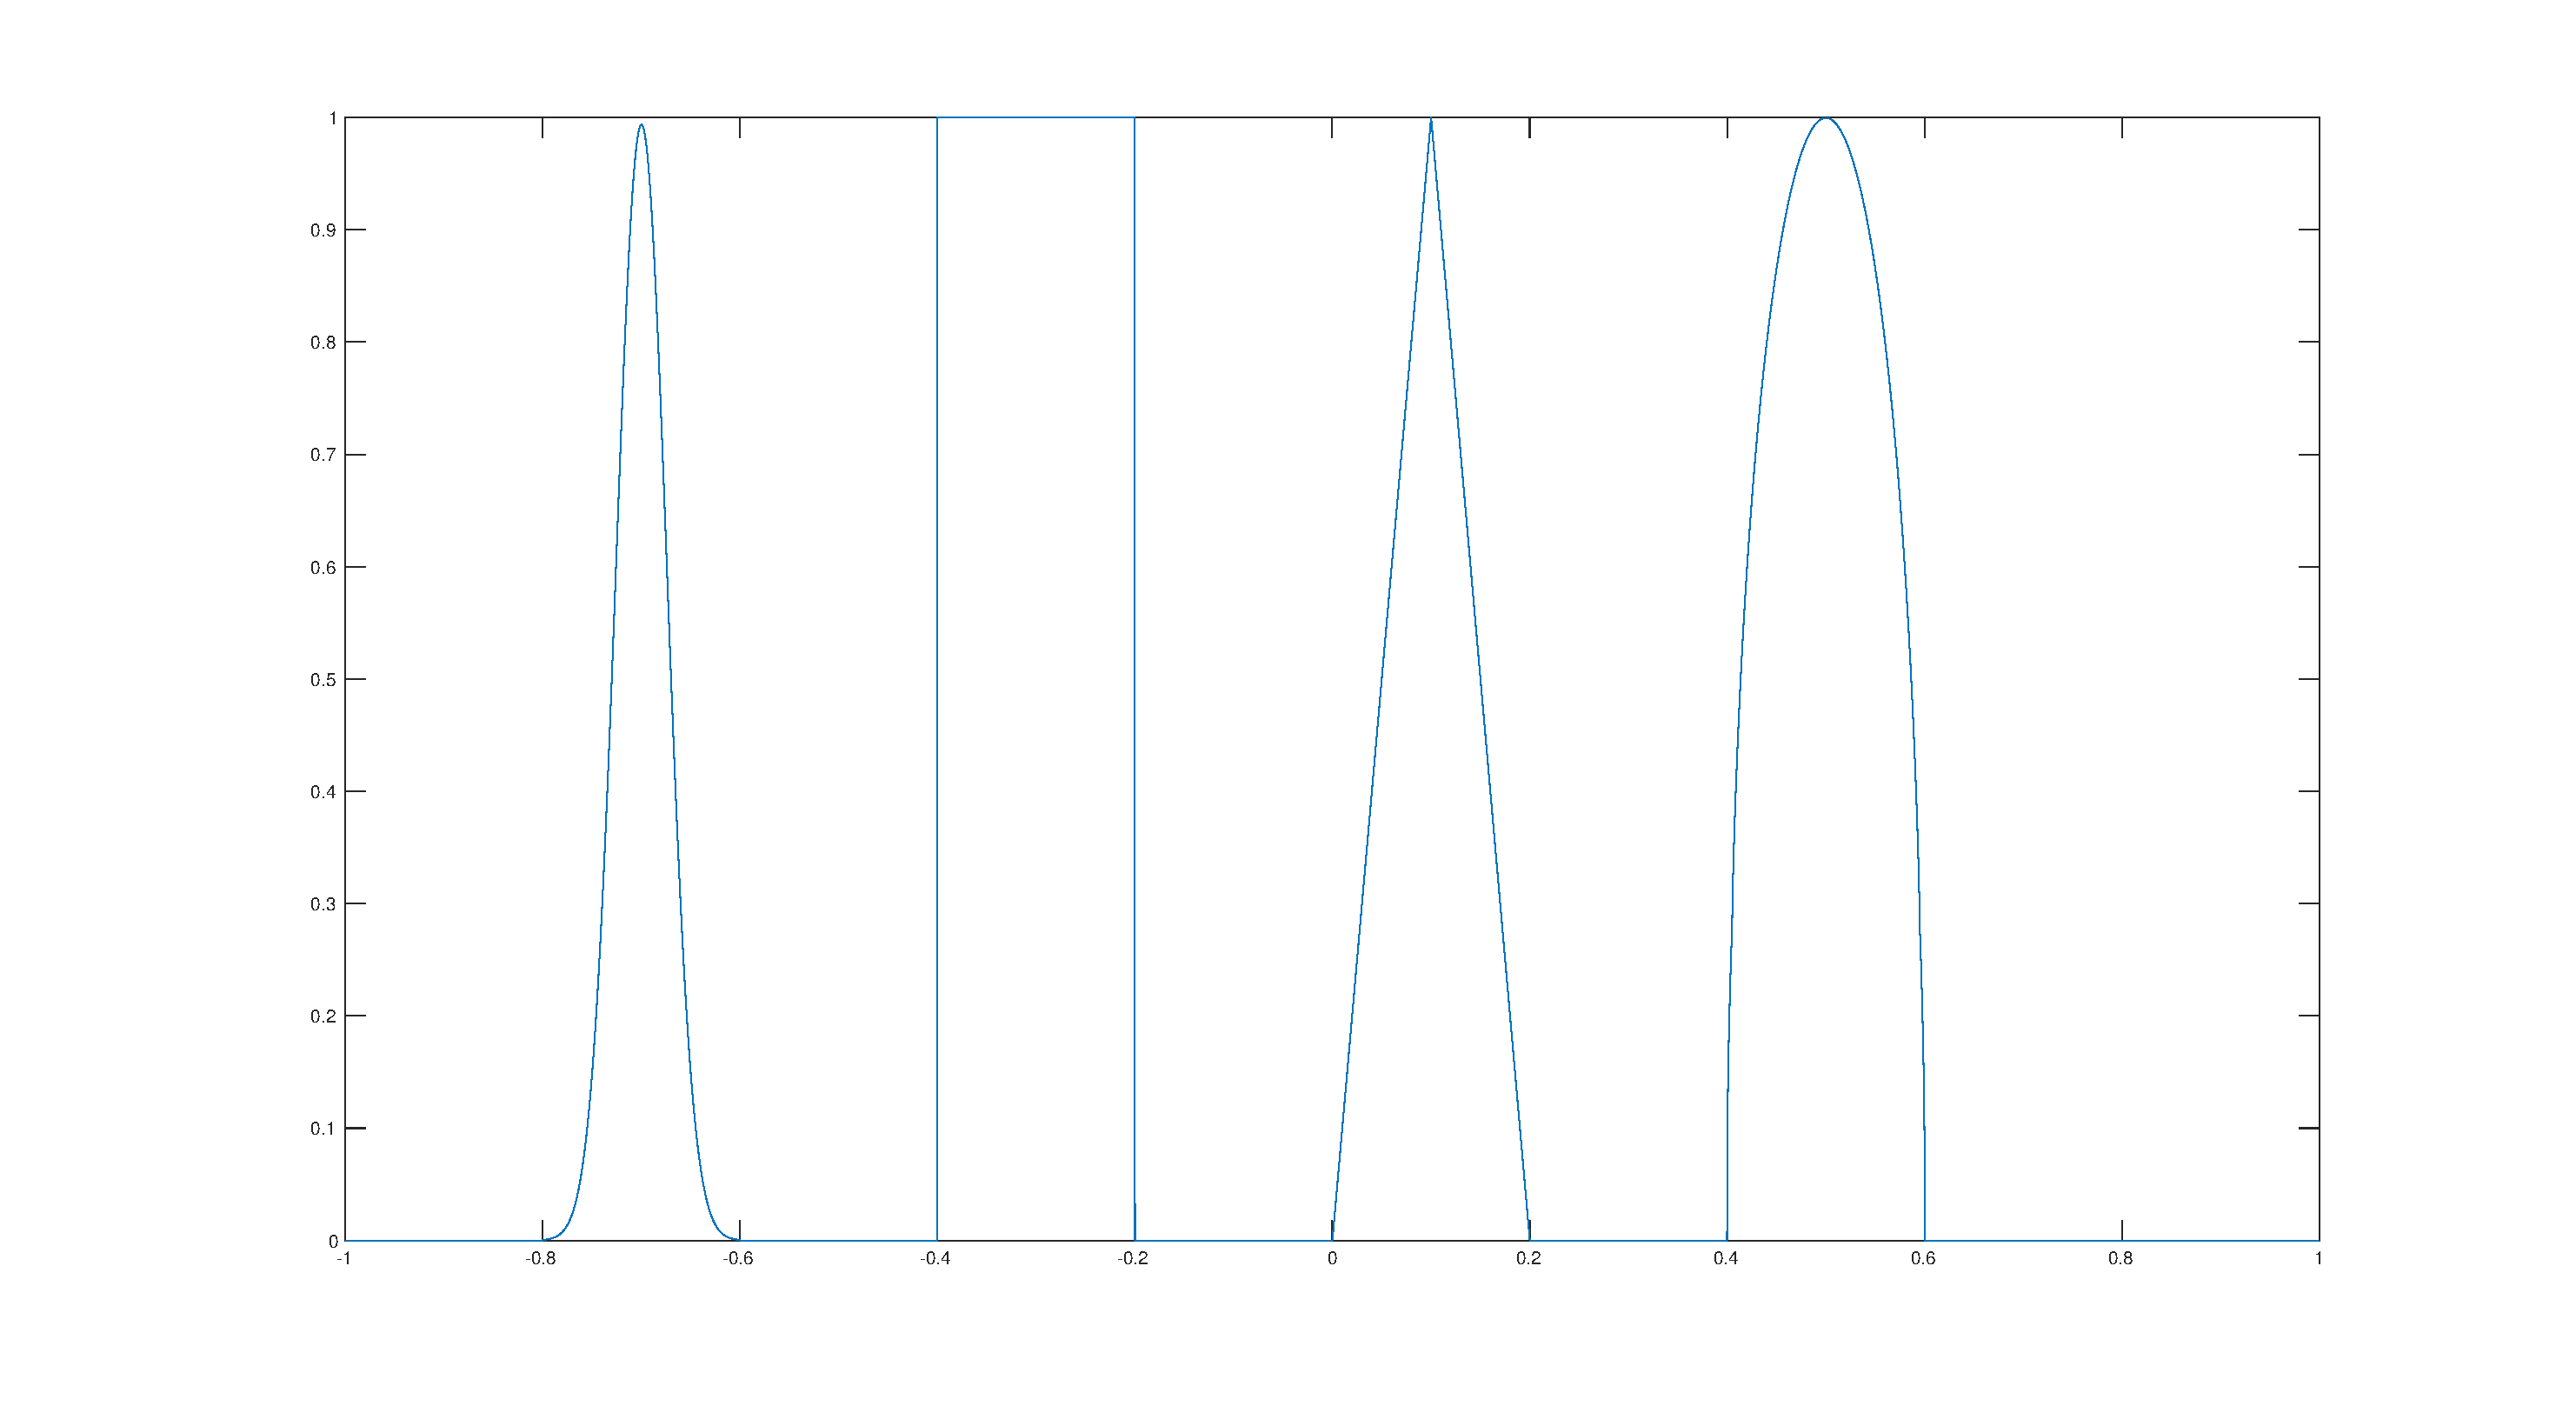
\includegraphics[width=\textwidth]{./images/advection_t0.eps}
  \end{center}
  \caption{初始值}
\end{figure}
终止时刻$t=8$,可以预期真解与初始值是一致的。
本数值实验的$N=10000,CFL=0.6$,时间方向采用3阶RK,边界采用周期边界条件。
\newpage
以下为不同通量的计算结果,:
\begin{figure}[H]
  \subfigure[LF]{
    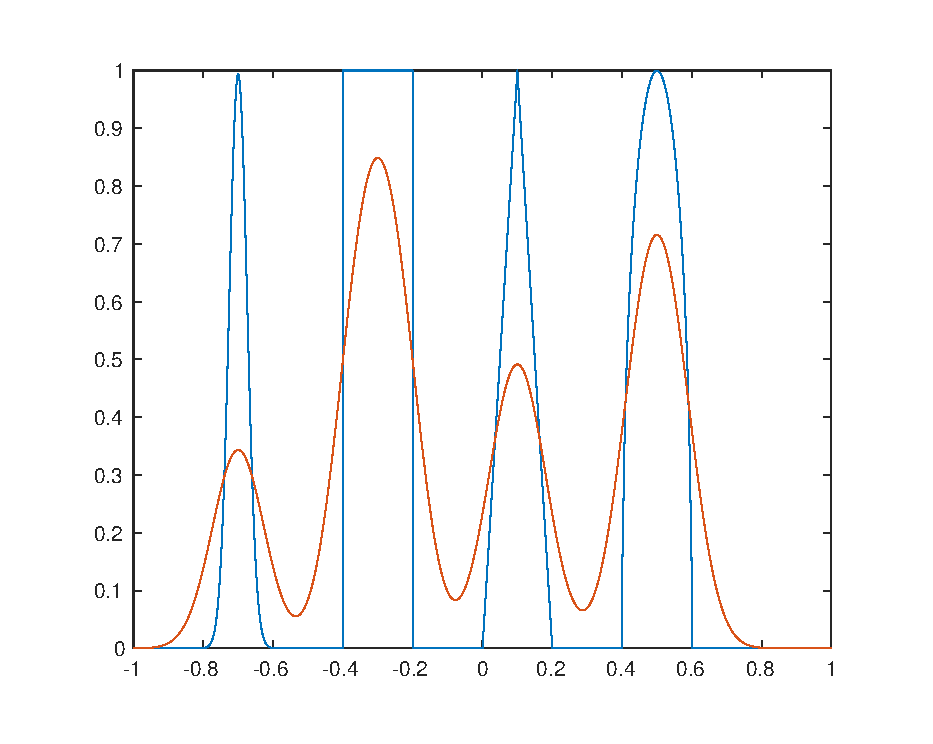
\includegraphics[width=0.45\textwidth, height=0.225\textheight]{./images/advection_LF.eps}
  }
  \subfigure[LW]{
    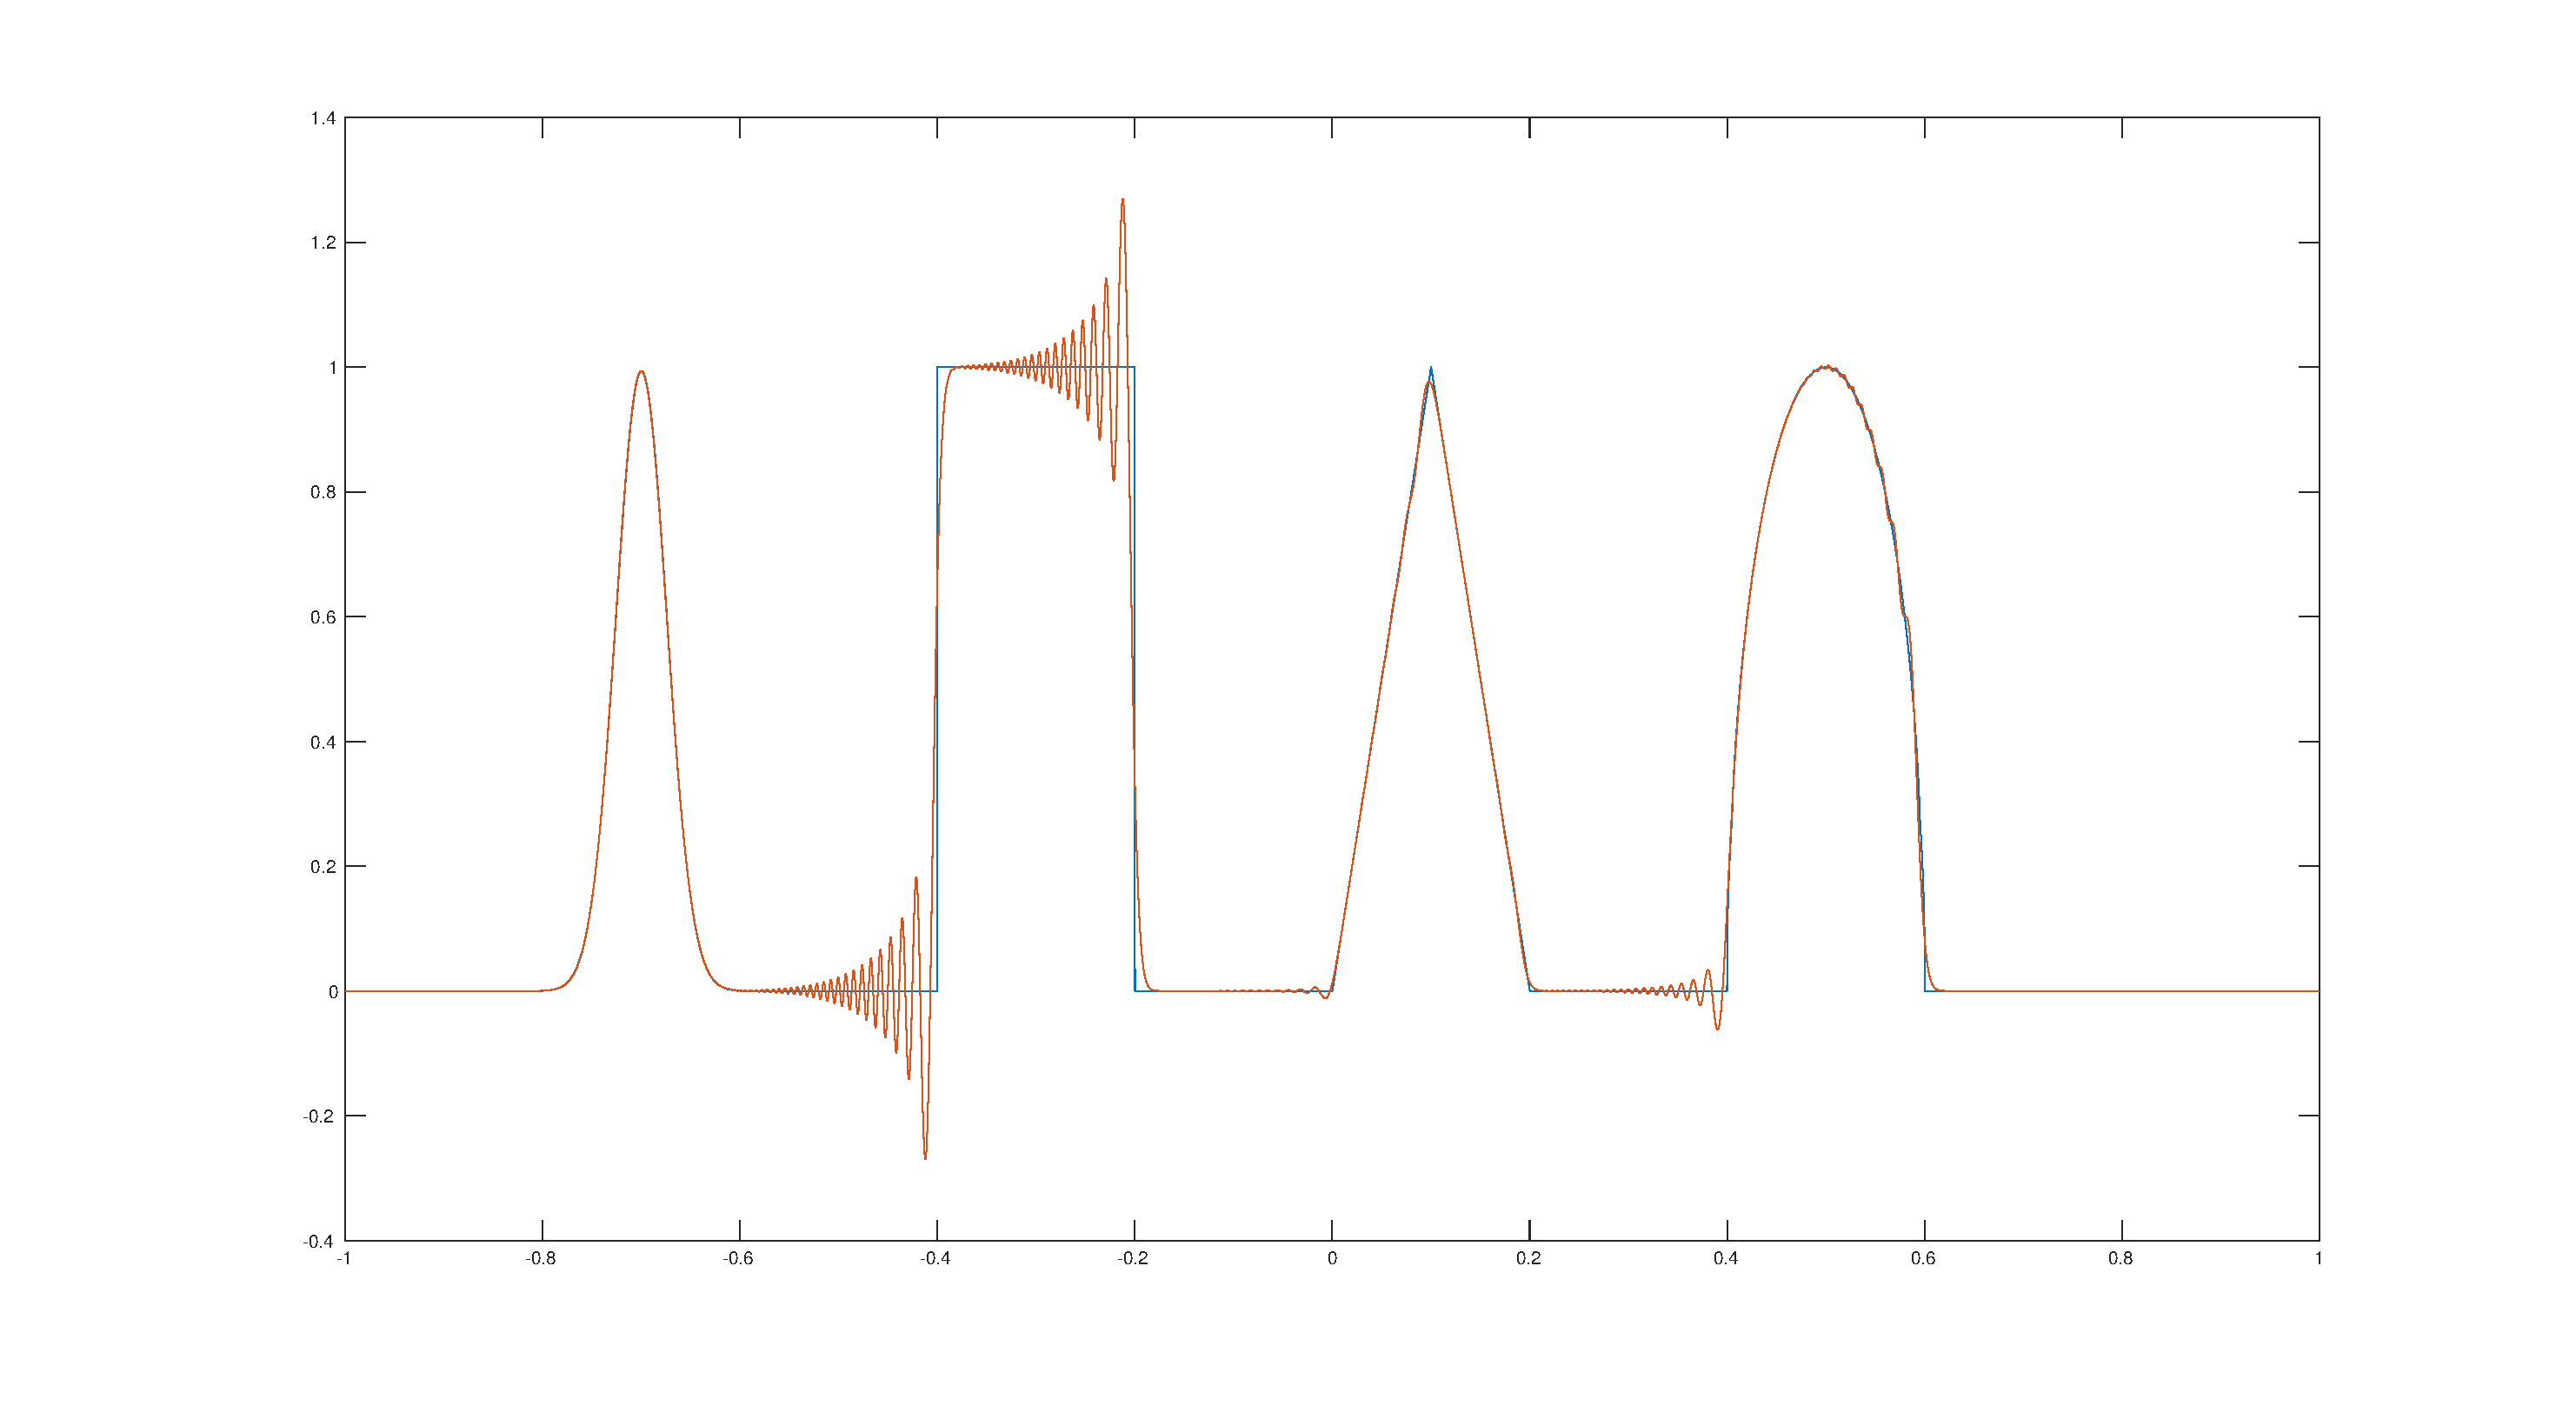
\includegraphics[width=0.45\textwidth,height=0.225\textheight]{./images/advection_LW.eps}
  }
  \subfigure[Force]{
    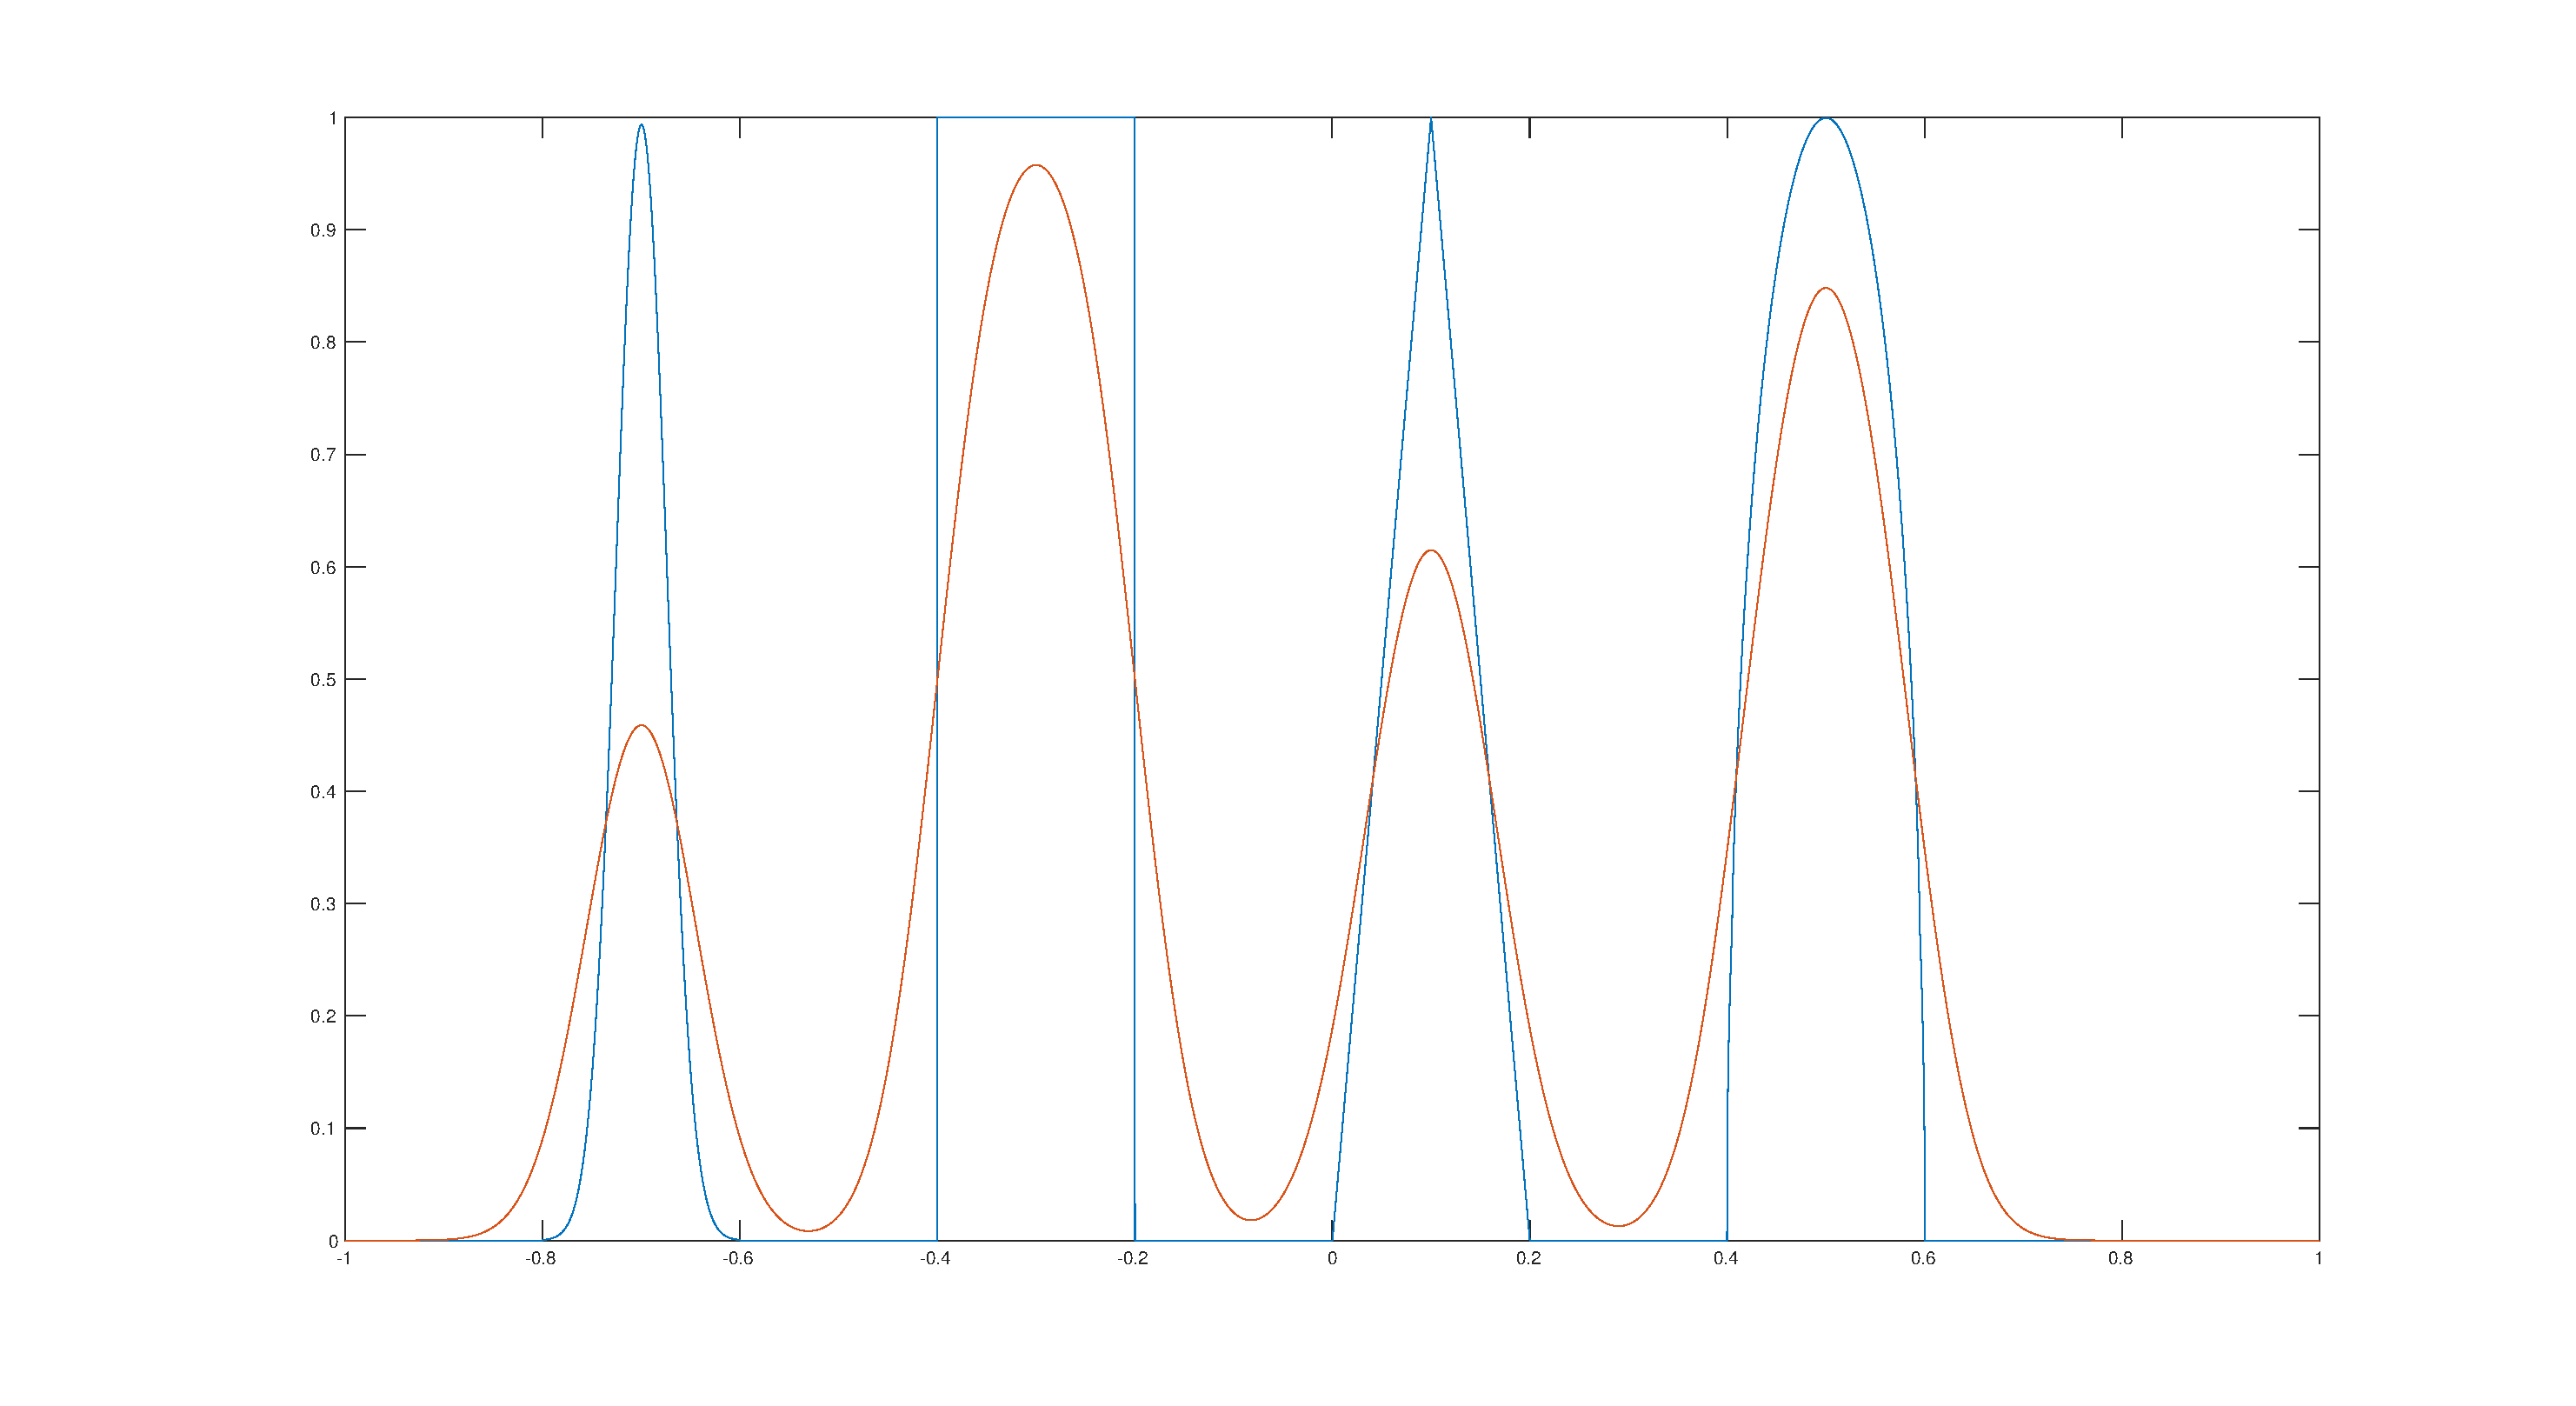
\includegraphics[width=0.45\textwidth,height=0.225\textheight]{./images/advection_Force.eps}
  }
  \subfigure[Godunov]{
    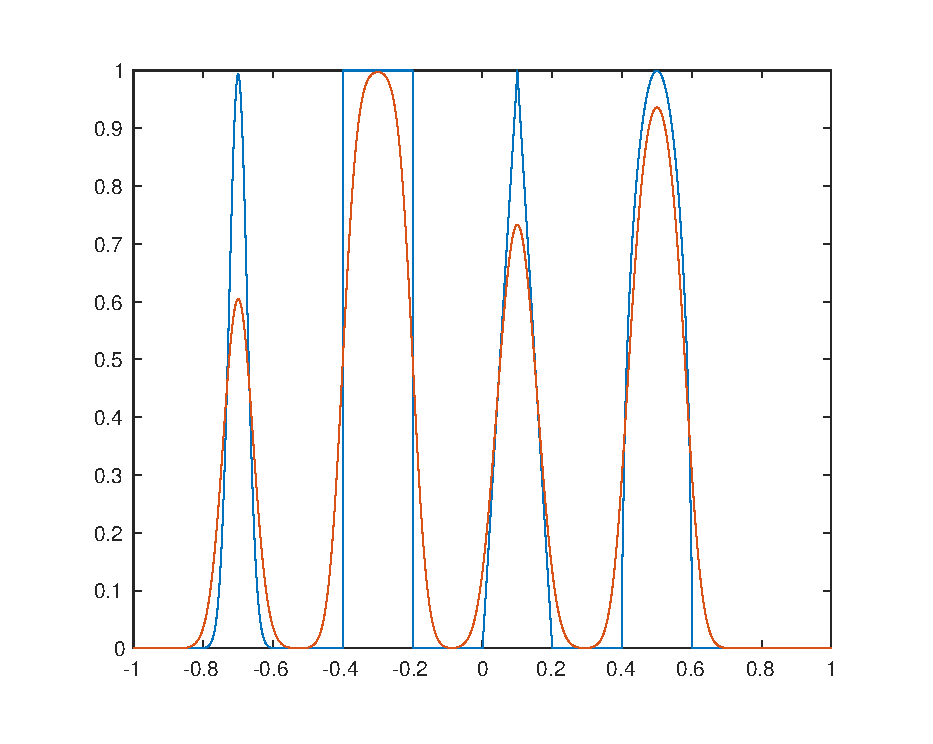
\includegraphics[width=0.45\textwidth,height=0.225\textheight]{./images/advection_Godunov.eps}
  }
\end{figure}
对以上结果做一个总结:
\begin{itemize}
  \item Lax-Friedrich格式数值通量较为保守,它是一个TVD的数值通量,没有
    震荡,但耗散较大。
  \item Lax-Wendroff格式数值通量是一个二阶的数值通量,对于光滑部分处理
    的较好,没有耗散,但在间断处会出现数值震荡。
  \item Force格式数值通量是对LF和LW的平均,而G-Force是对它们的加权平均
    。从数值结果来看,这一处理能减少数值耗散,但整体耗散还是过大。
  \item 对于线性对流问题,Godunov,HLL,HLLC通量的表达式一致,耗散来说较
    小,但依旧不足以令人满意。
\end{itemize}
\newpage
上述结果说明对数据进行线性重构必不可少。

以下是Lax-Friedrich格式数值通量在不同重构下的表现:
\begin{figure}[H]
  \subfigure[LF-minmod]{
    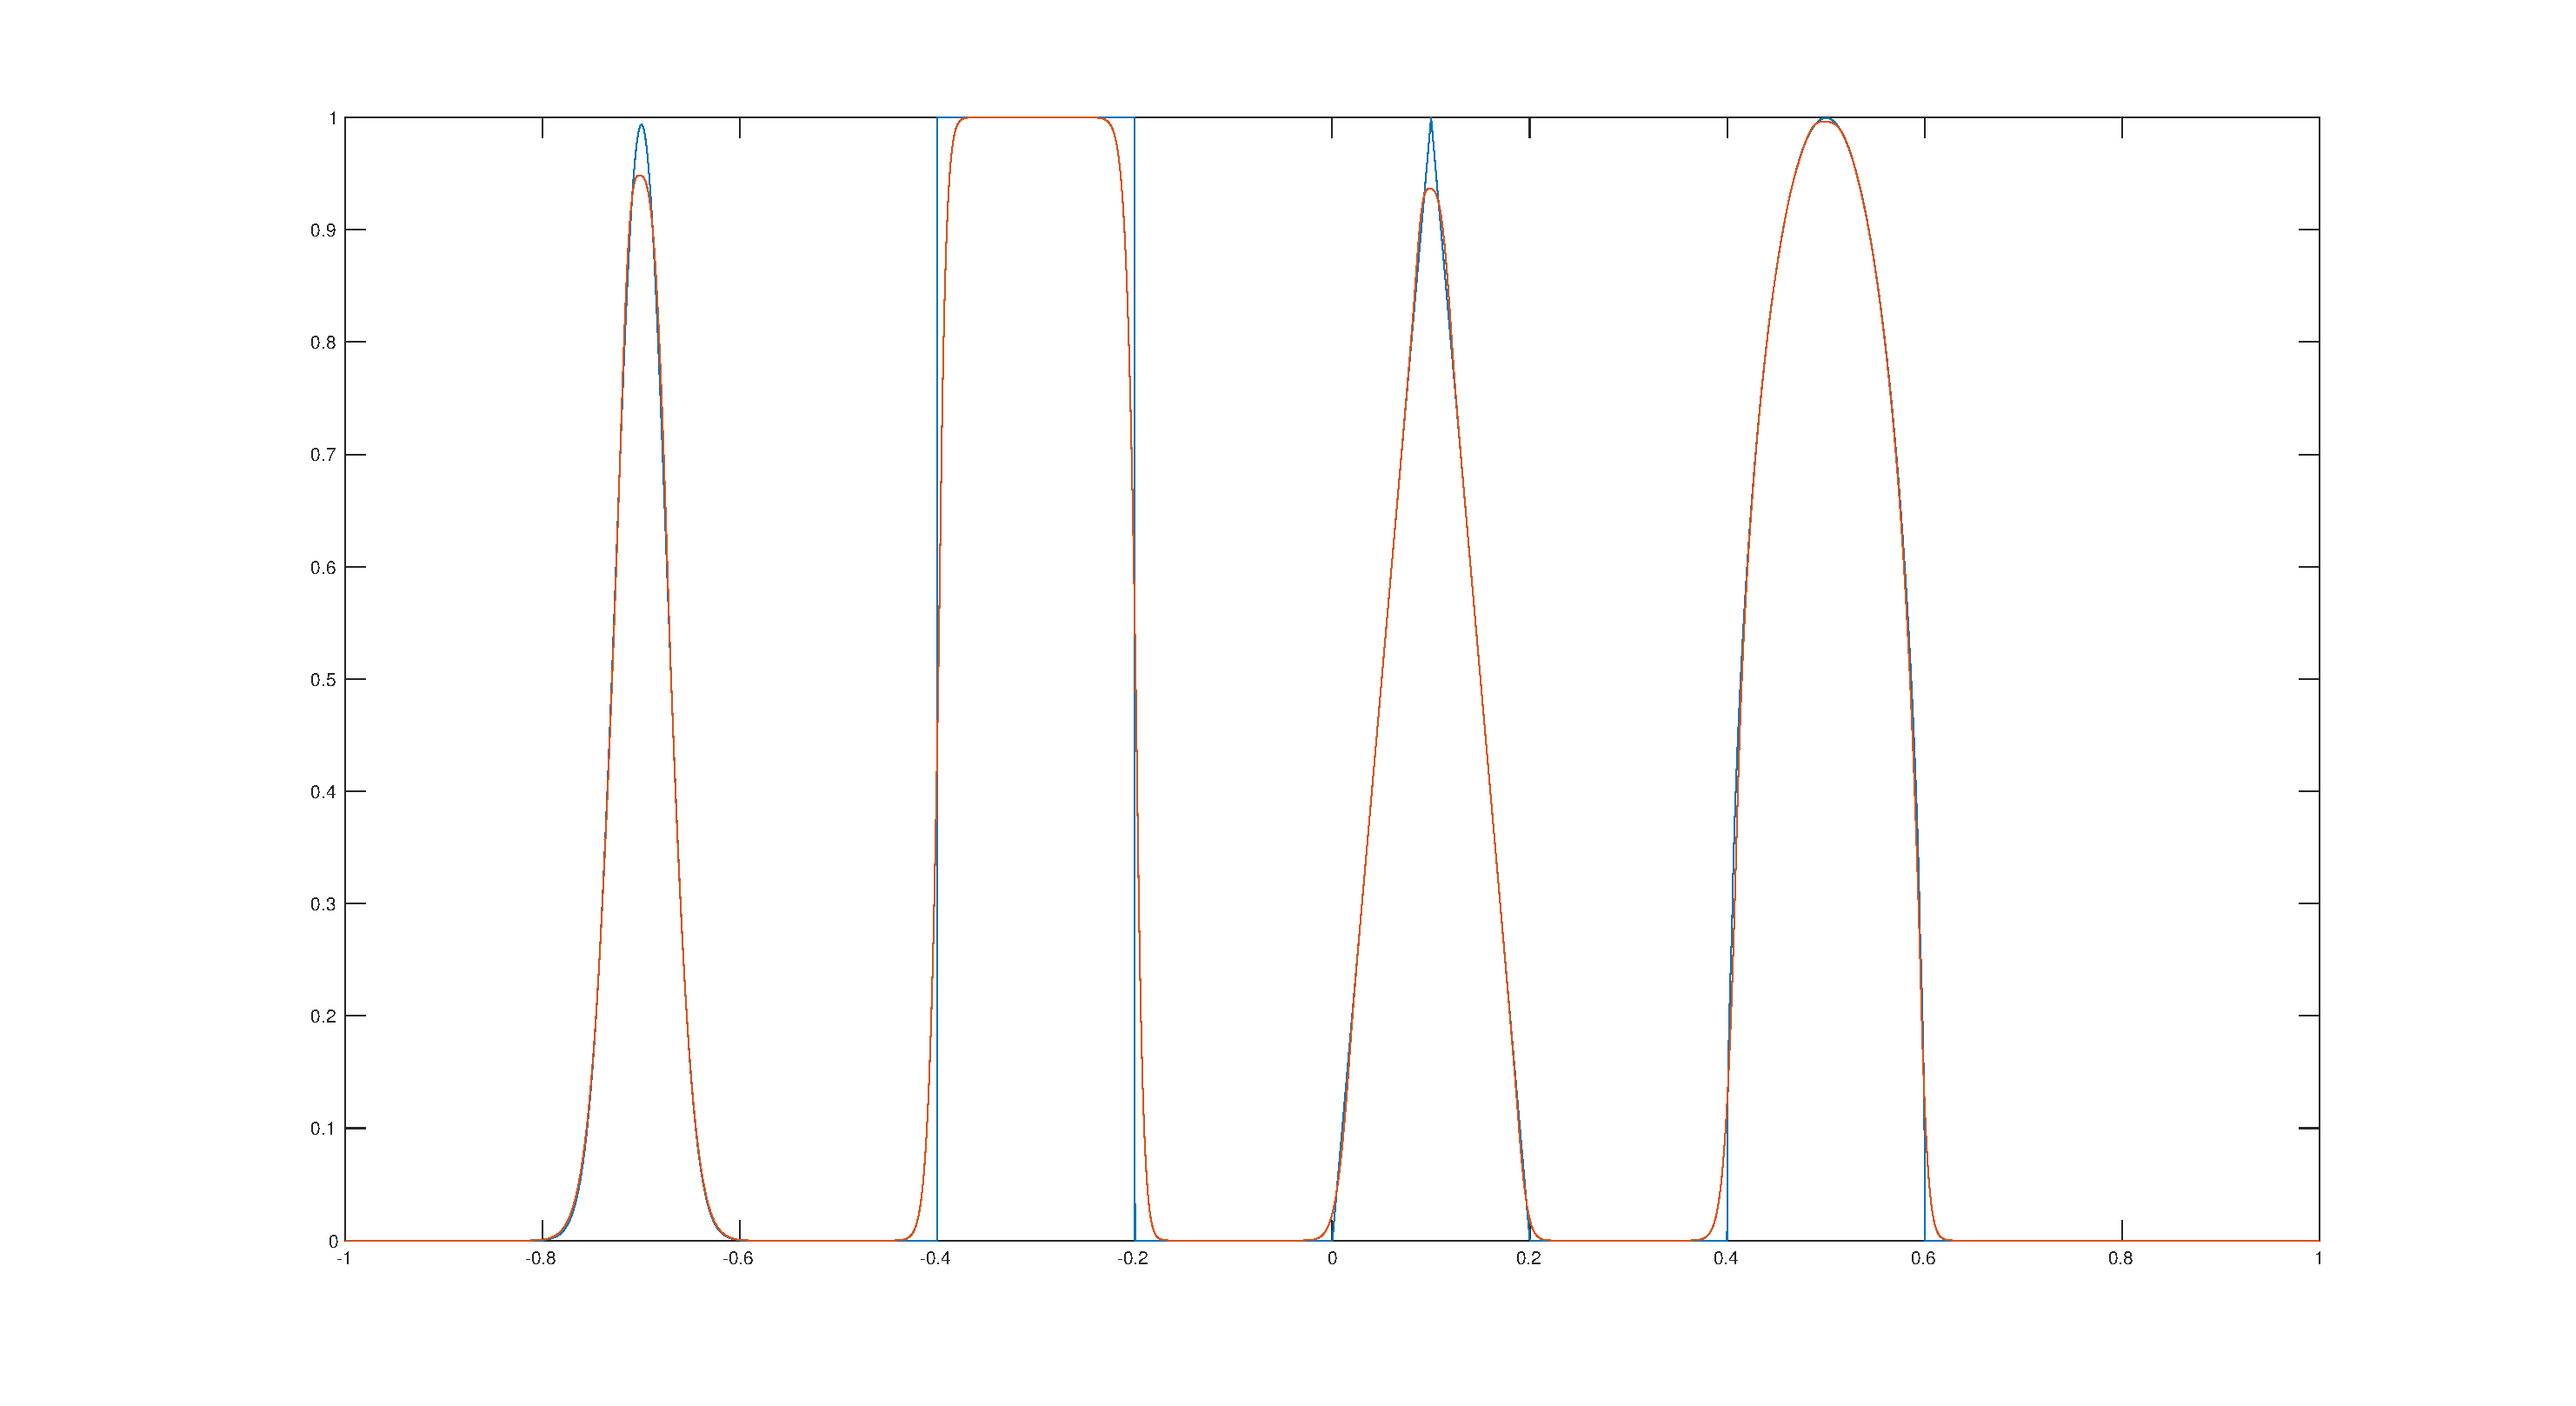
\includegraphics[width=0.45\textwidth,height=0.225\textheight]{./images/advection_LF_minmod_RK3.eps}
  }
  \subfigure[LF-superbee]{
    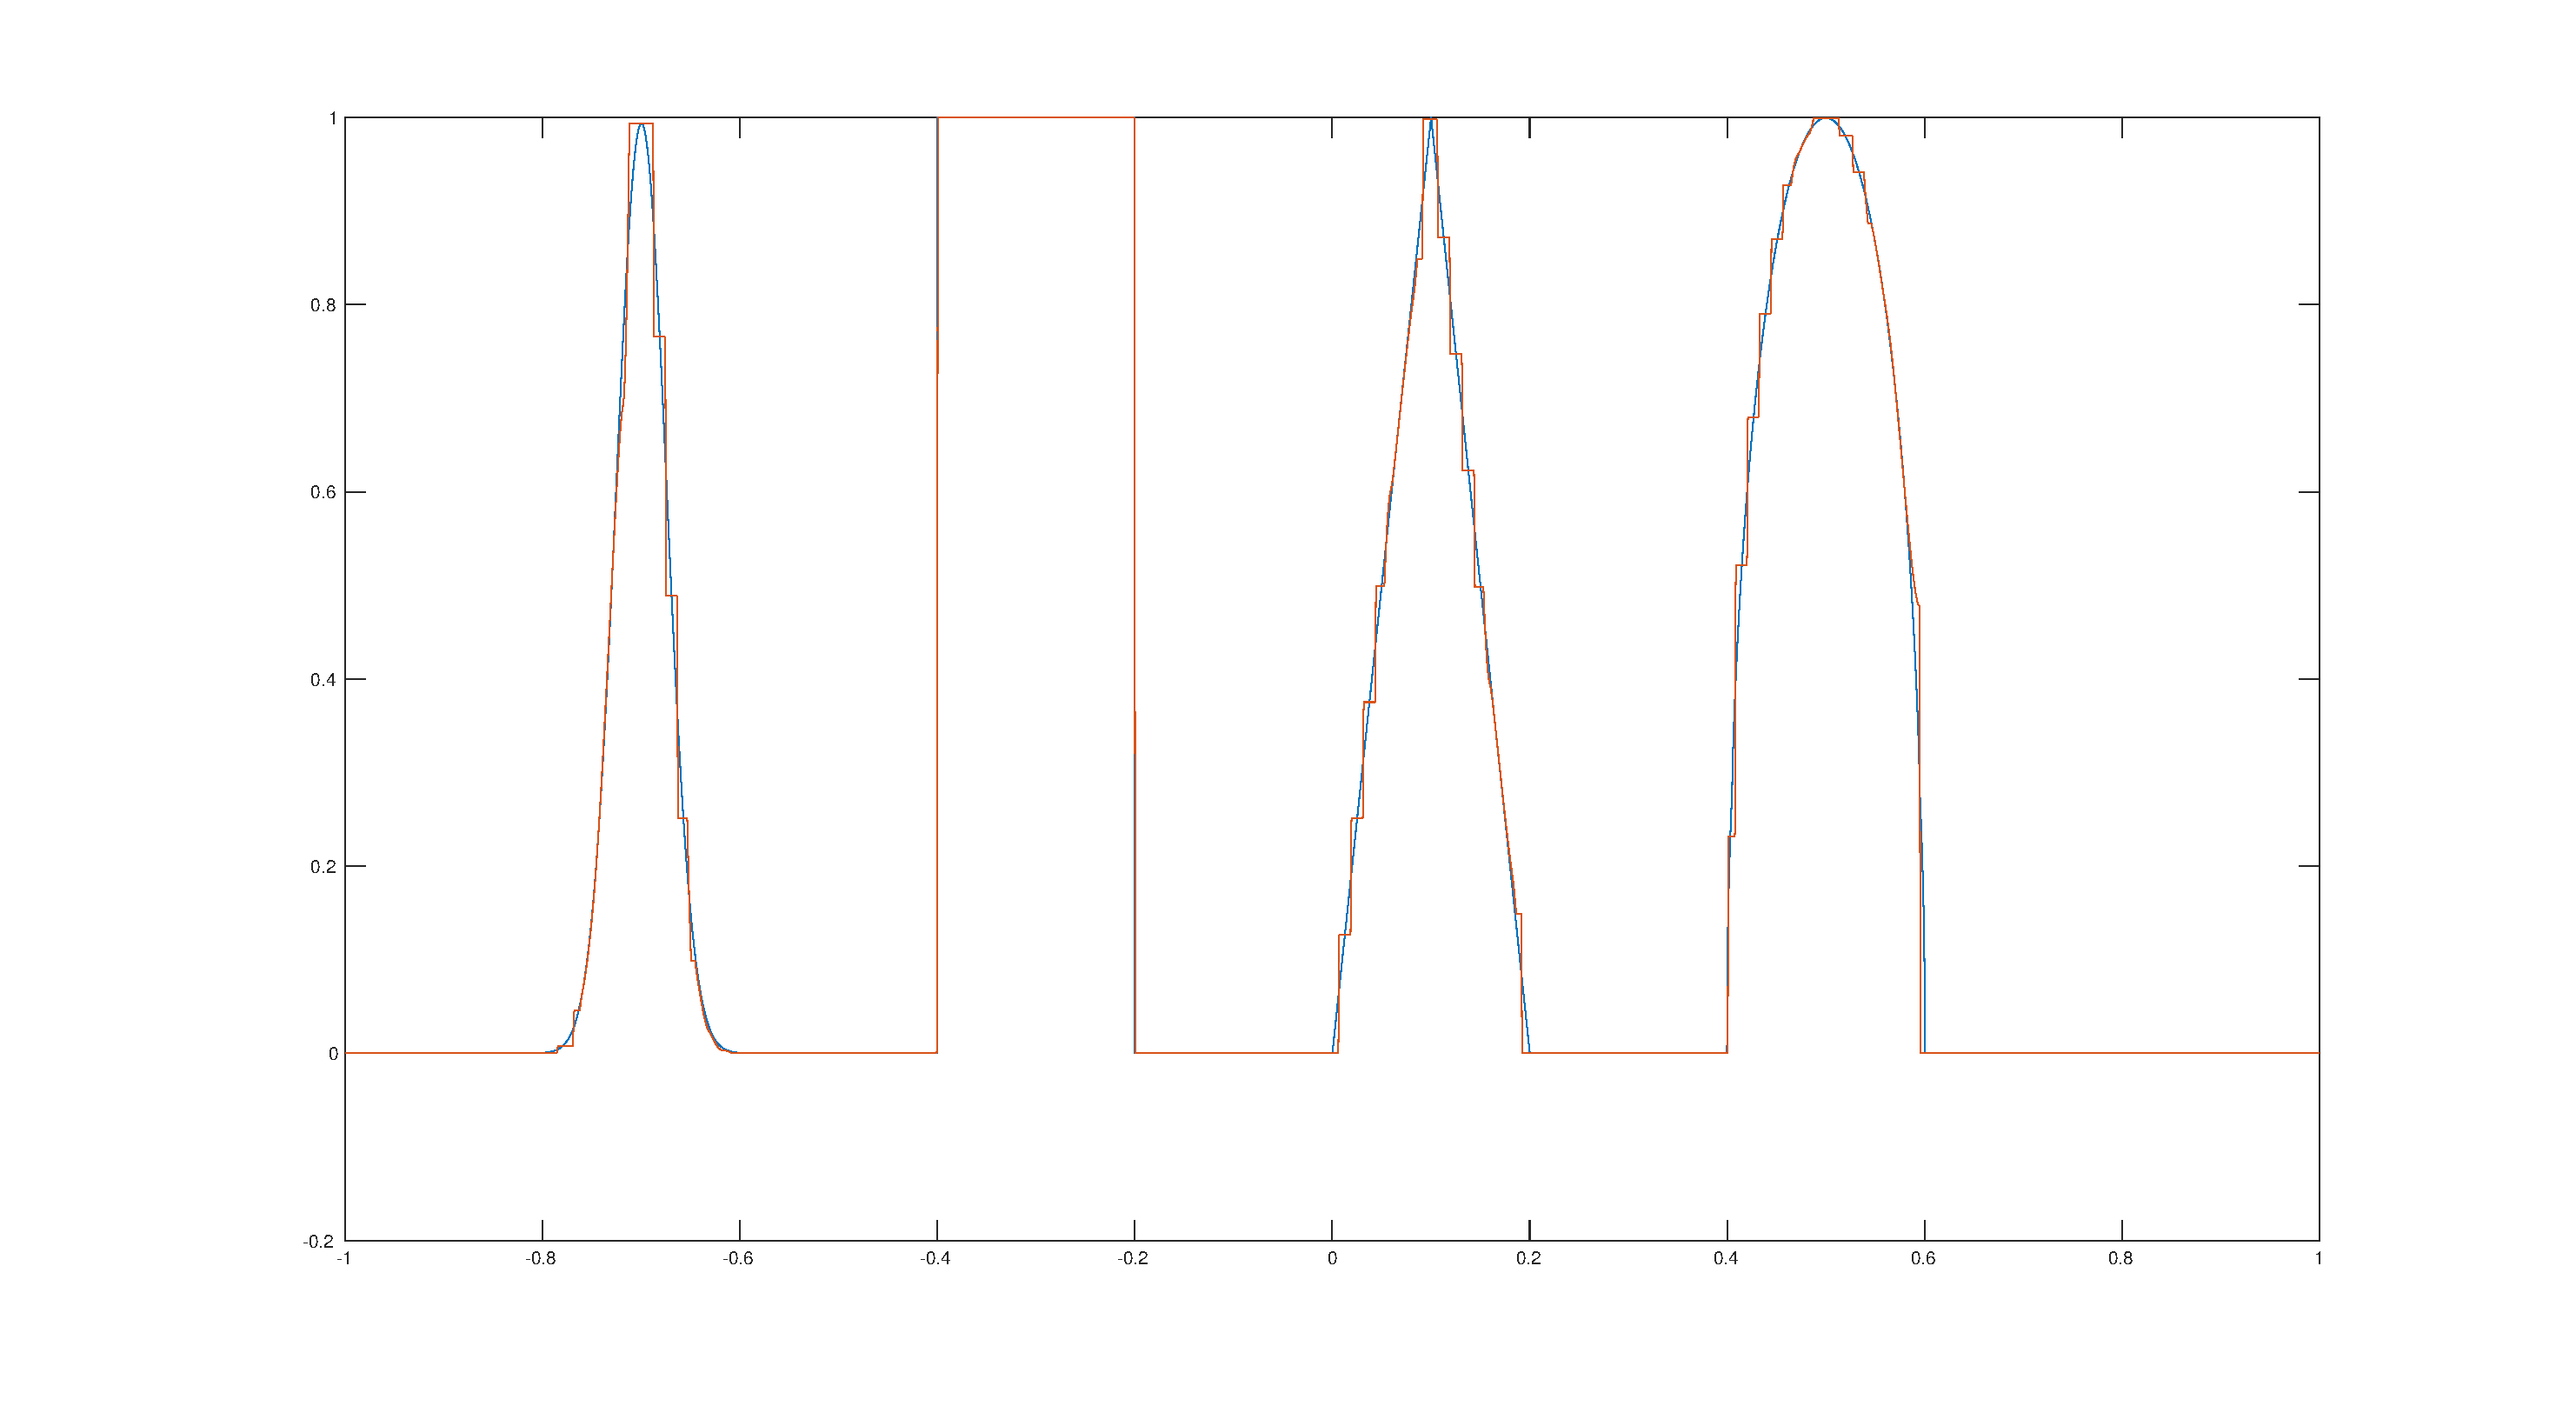
\includegraphics[width=0.45\textwidth,height=0.225\textheight]{./images/advection_LF_superbee_RK3.eps}
    }
  \subfigure[LF-MC]{
    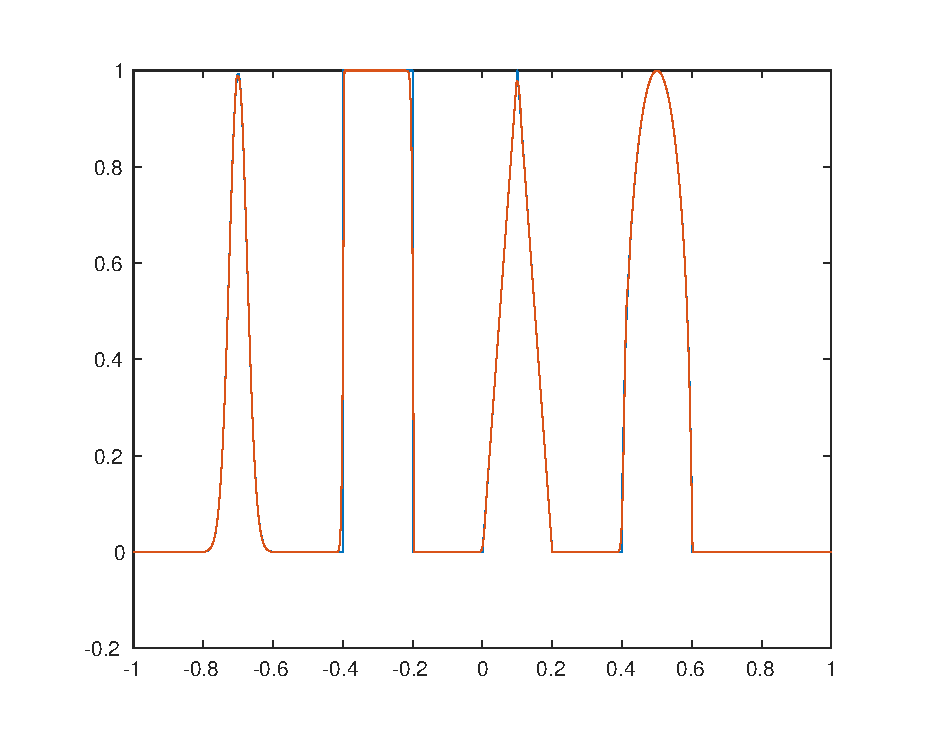
\includegraphics[width=0.45\textwidth,height=0.225\textheight]{./images/advection_LF_MC_RK3.eps}
  }
  \hspace{1cm}
  \subfigure[LF-vanLeer]{
    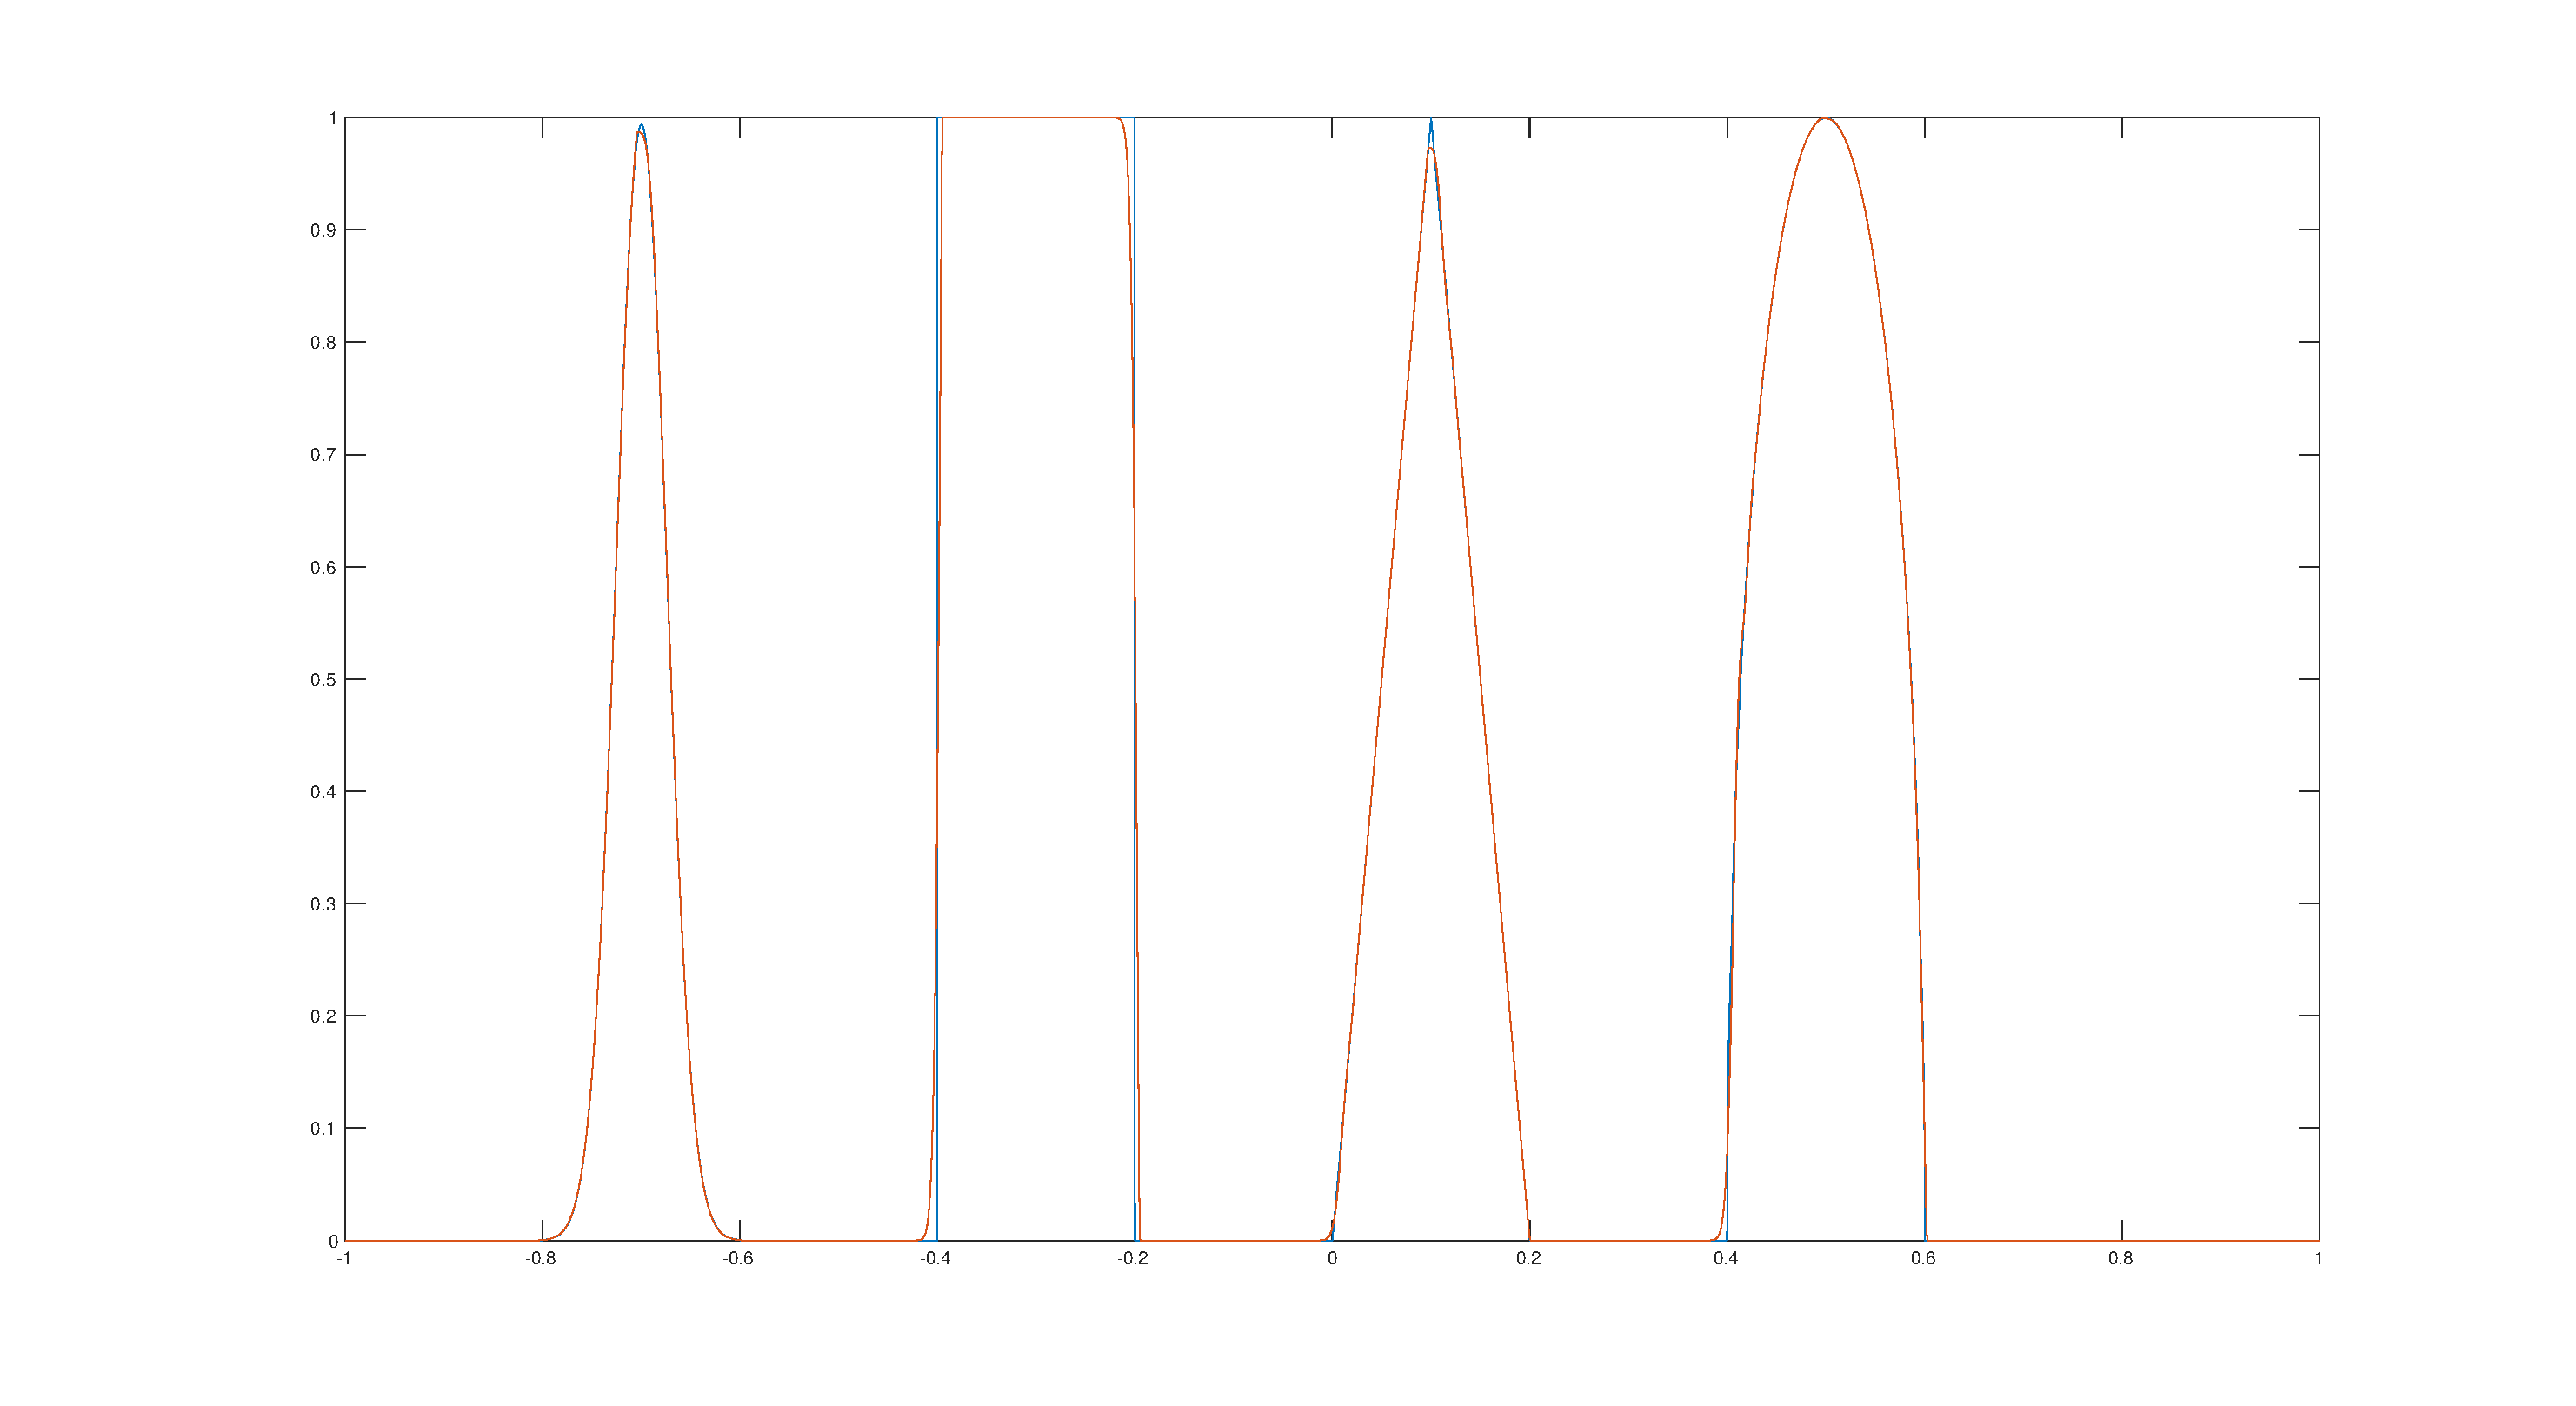
\includegraphics[width=0.45\textwidth,height=0.225\textheight]{./images/advection_LF_vanLeer_RK3.eps}
  }
\end{figure}
对以上结果做一个总结:
\begin{itemize}
  \item 斜率限制器方法能够有效的去除耗散
  \item minmod斜率限制器较为保守,是一个TVD的斜率限制器,根据数值结果
    来看其耗散最大。
  \item superbee是一个较为激进的斜率限制器,容易将其他波算成方波的效果
    ,从数值结果来看也不是保极值的。
  \item MC方法能够较好的逼近真实情况,但它也不是保极值的限制器。
  \item vanLeer限制器的数值结果与MC限制器类似,而且是保极值的。
\end{itemize}
\newpage 
下图为Lax-Wendroff 数值通量在不同限制器下的效果。
\begin{figure}[H]
  \begin{center}
    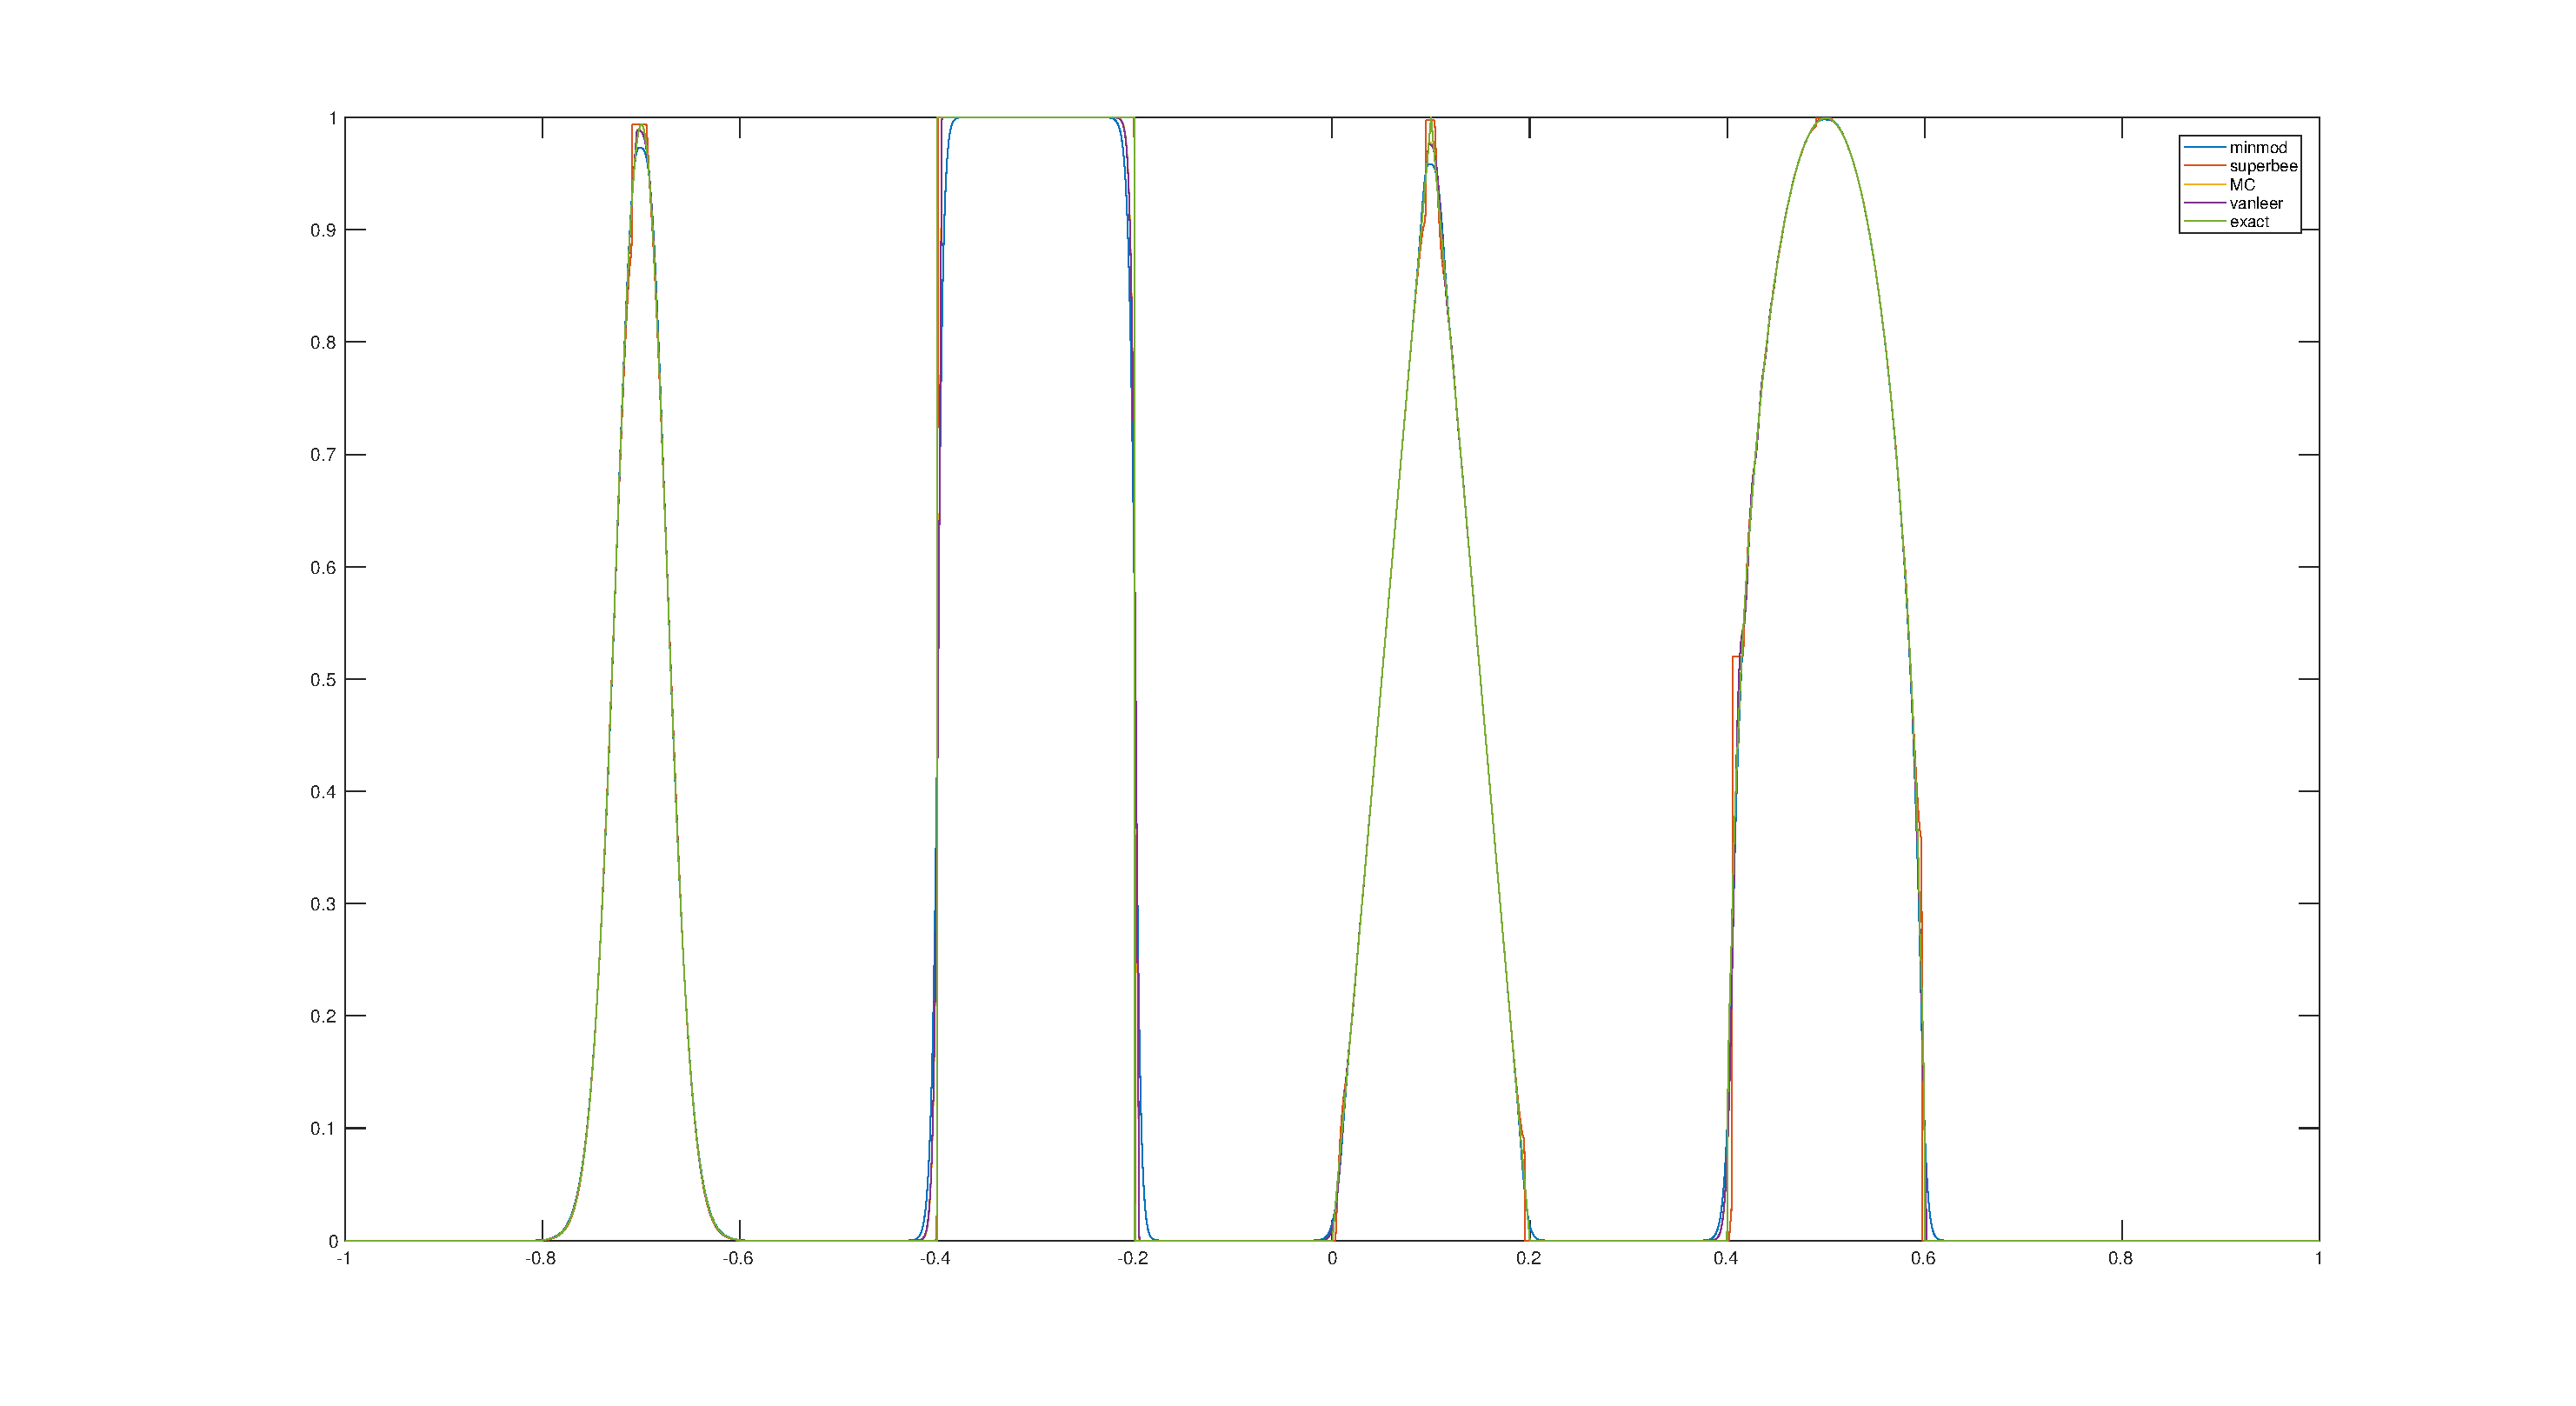
\includegraphics[width=\textwidth]{./images/advection_LW_all.eps}
  \end{center}
  \caption{LW格式下各种限制器效果}
\end{figure}
可见采用斜率限制器方法也能有效去除震荡,但除了minmod之外,其他限制器都
会出现非TVD的问题。
\subsubsection{Osher-Shu问题}
Osher-Shu问题的方程为1维Euler方程,其初值为:
\[(\rho,u,p)=\left\{
 \begin{aligned}
  & (3.857143,2.629369,10.33333), \quad & x < -4, \\
  & (1+0.2\sin(5x),0,1),\quad & x \geq -4. 
 \end{aligned}
 \right.
\]
我们这里的求解参数为$N=10000,t=1.8,CFL=0.6$,求解区域为$[-5,5]$,左侧
为入流边界条件,右侧为出流边界条件。

不加重构求解,各数值通量结果如下:
\begin{figure}[H]
  \begin{center}
    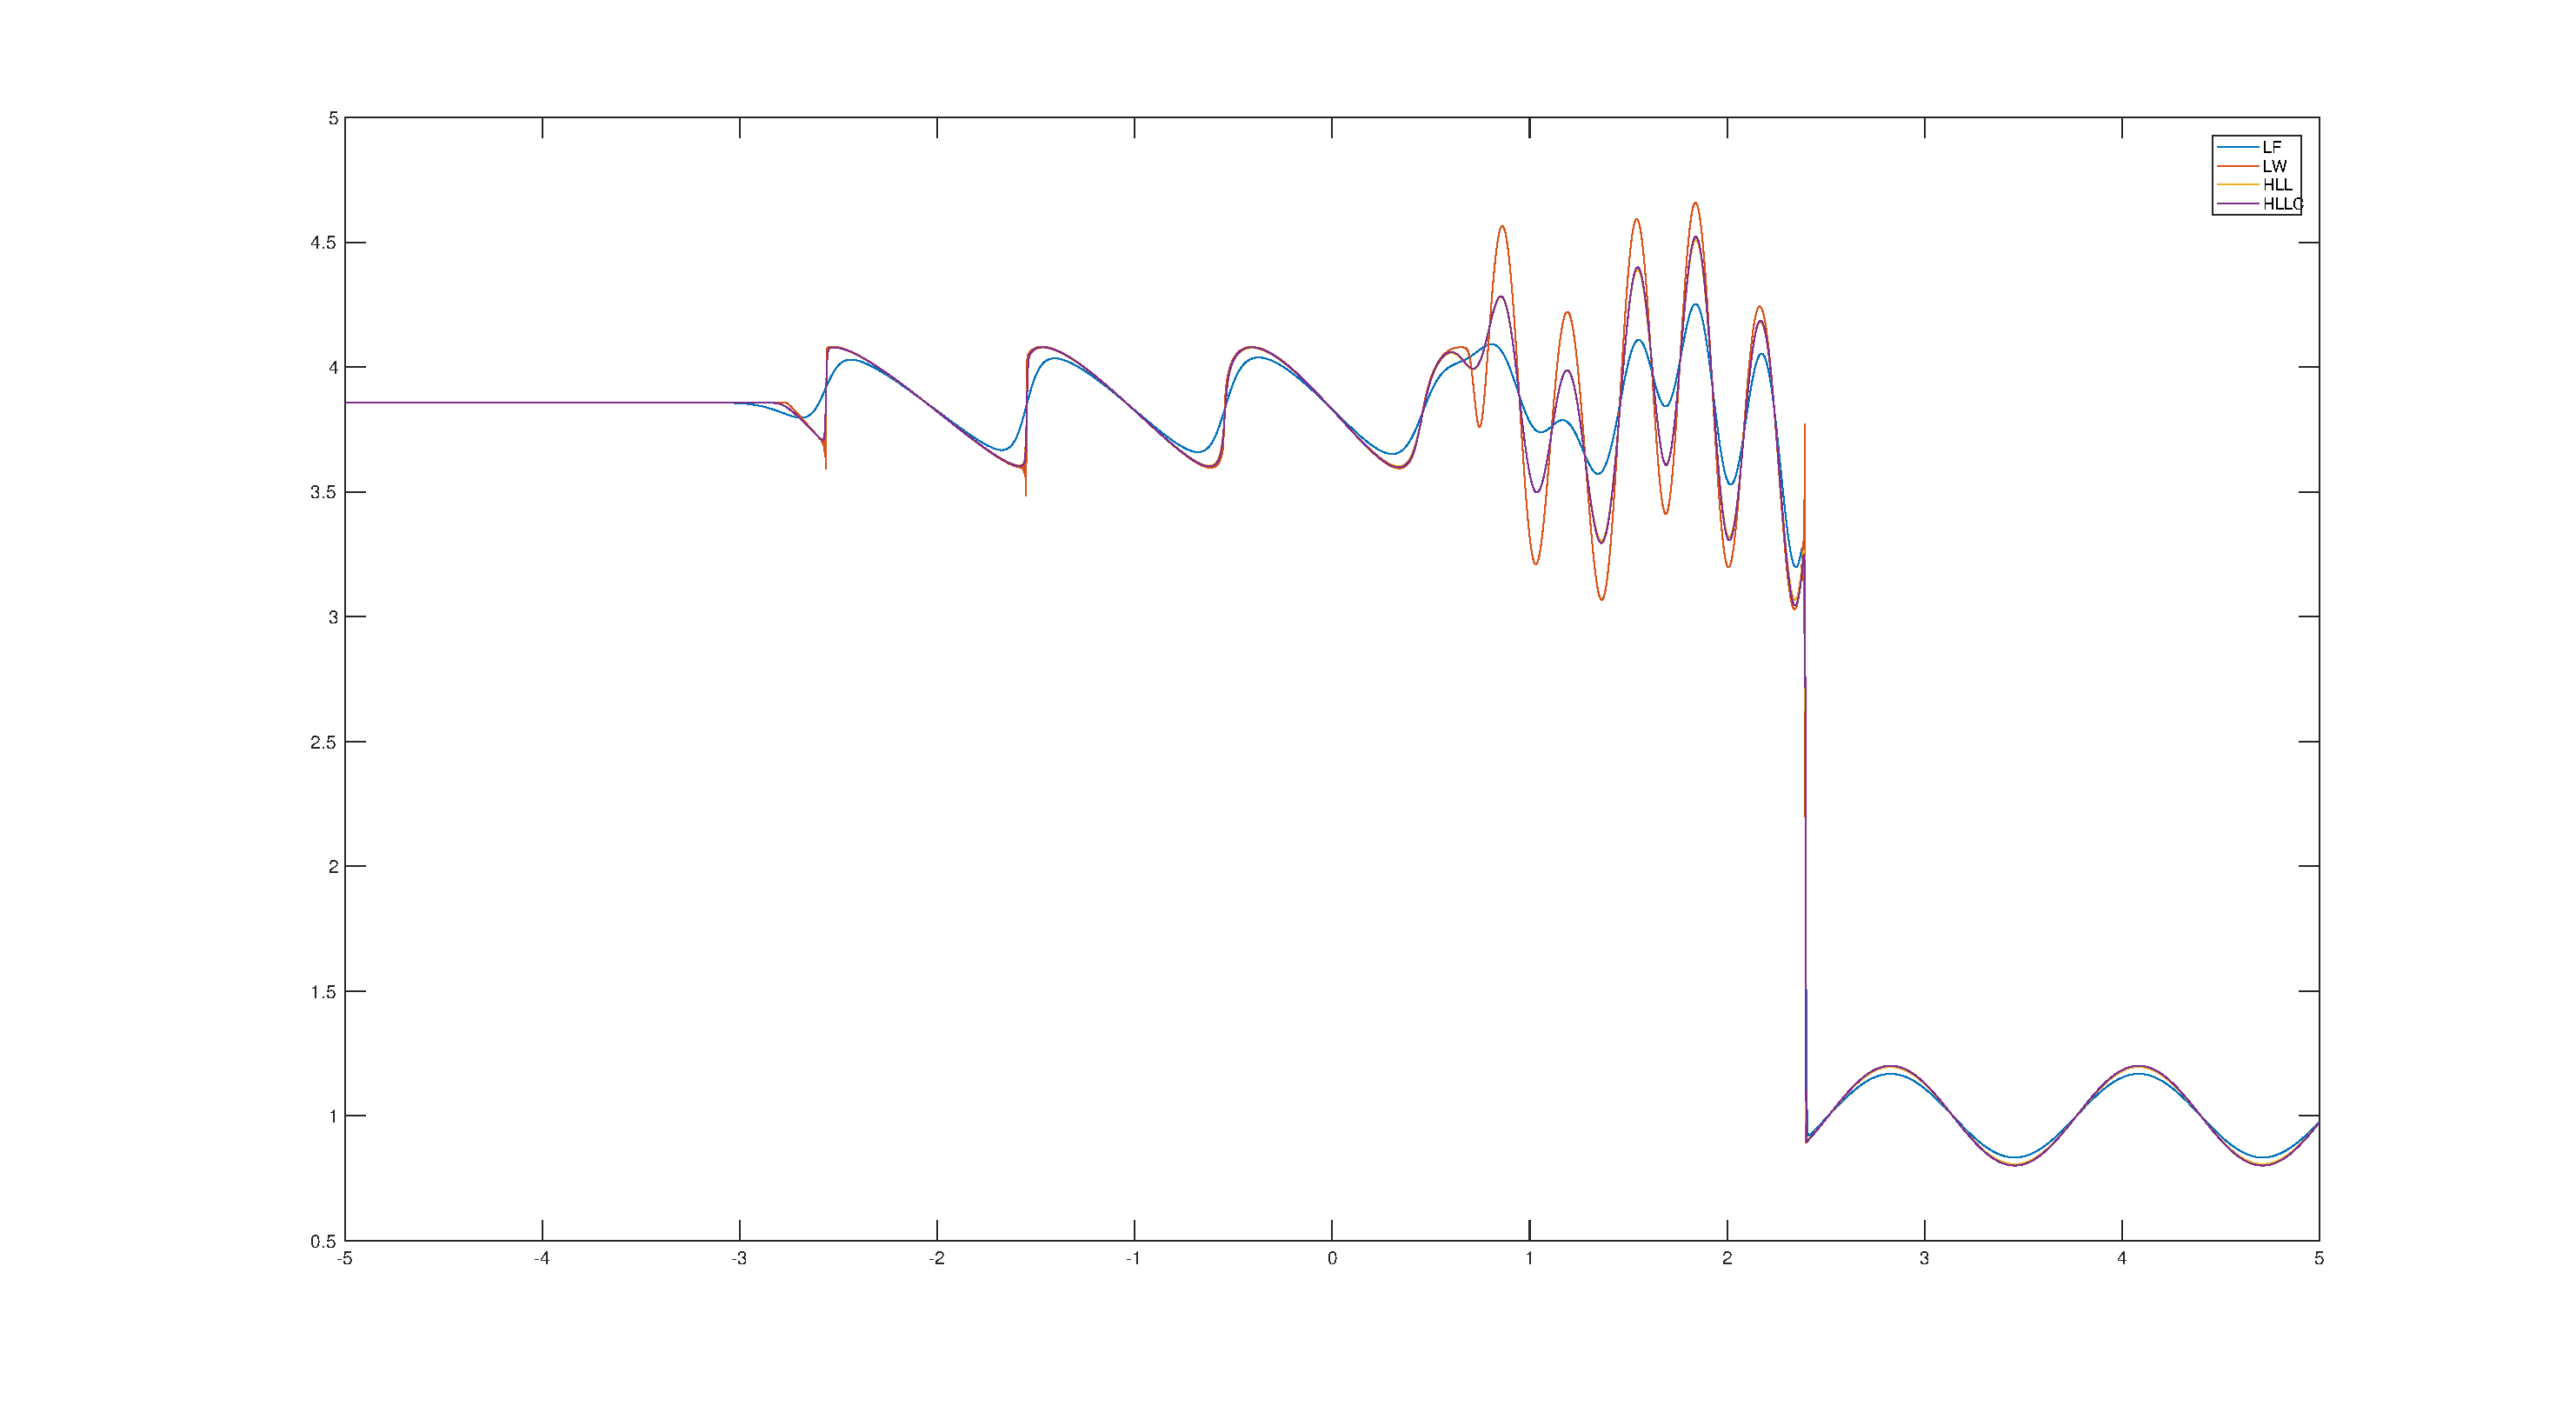
\includegraphics[width=\textwidth]{./images/EulerShu-Noreconstruction.eps}
    \caption{Osher-Shu问题,无重构}
  \end{center}
\end{figure}
可见在该问题下,LF数值通量还是体现了耗散大的问题,LW格式没有耗散,但有
数值震荡,HLL与HLLC格式类似,存在一定耗散。

\begin{figure}[H]
  \begin{center}
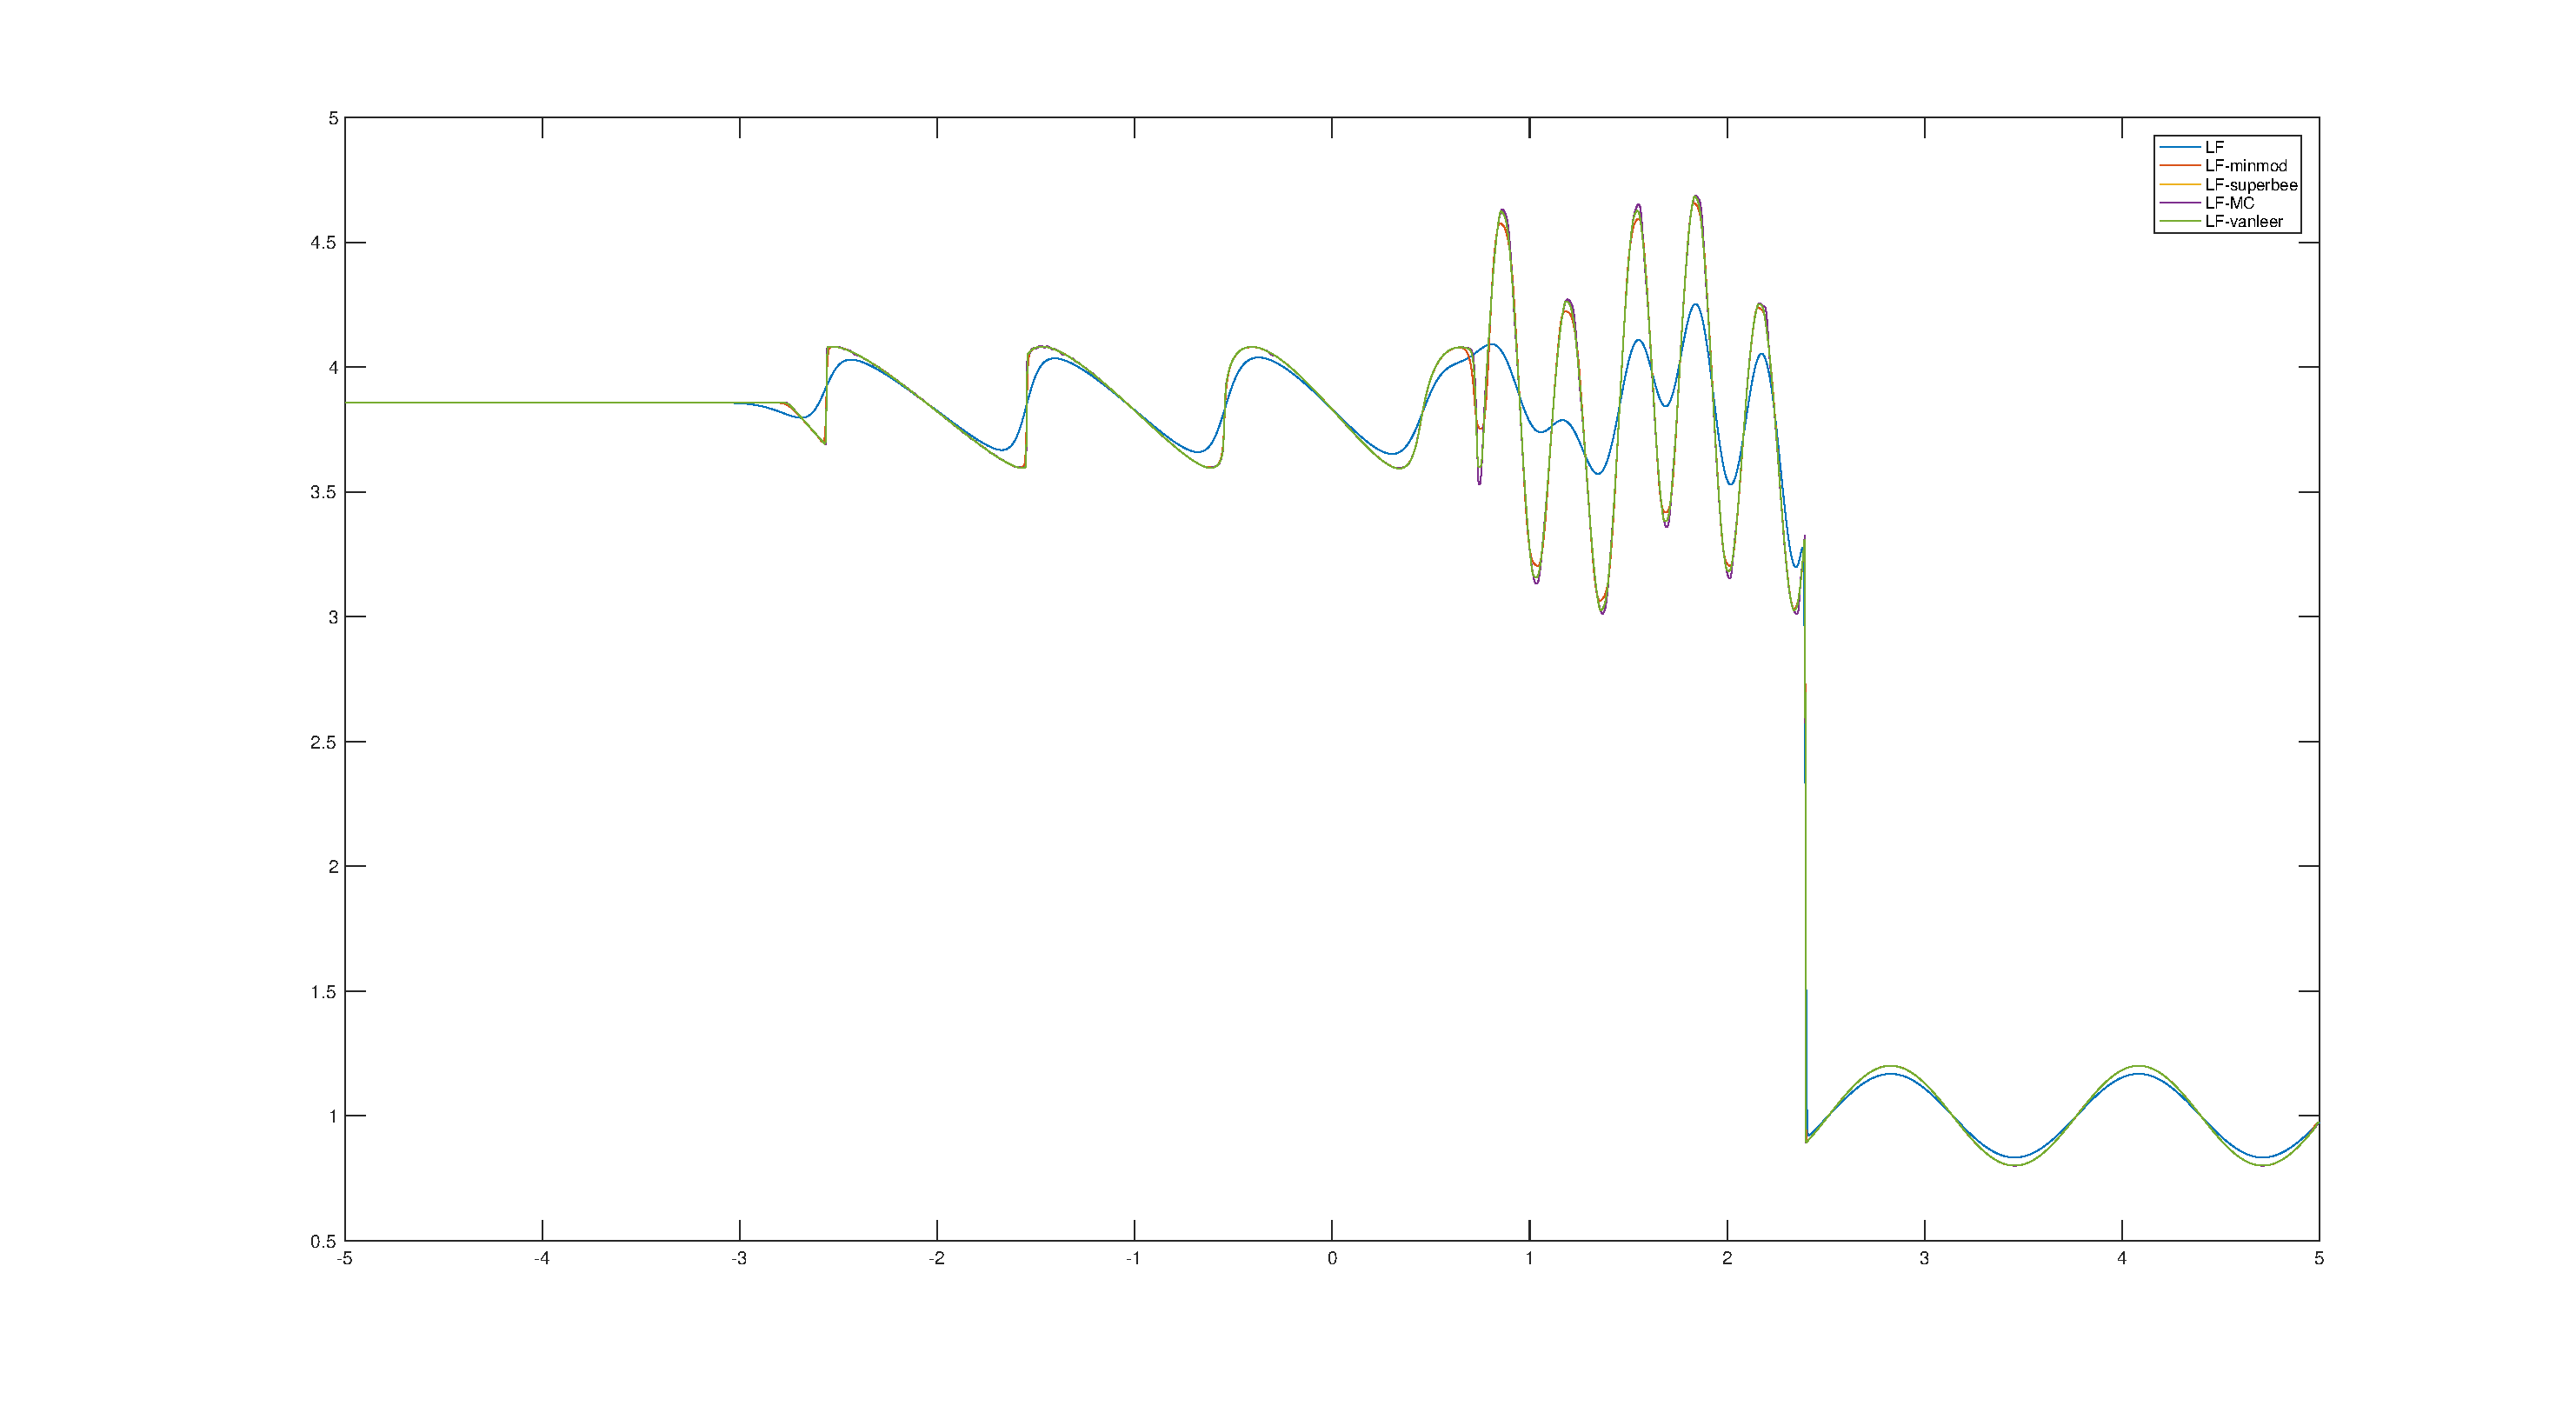
\includegraphics[width=\textwidth]{./images/EulerShu-LF.eps}
    \caption{Osher-Shu问题,LF数值通量}
  \end{center}
\end{figure}

\begin{figure}[H]
  \begin{center}
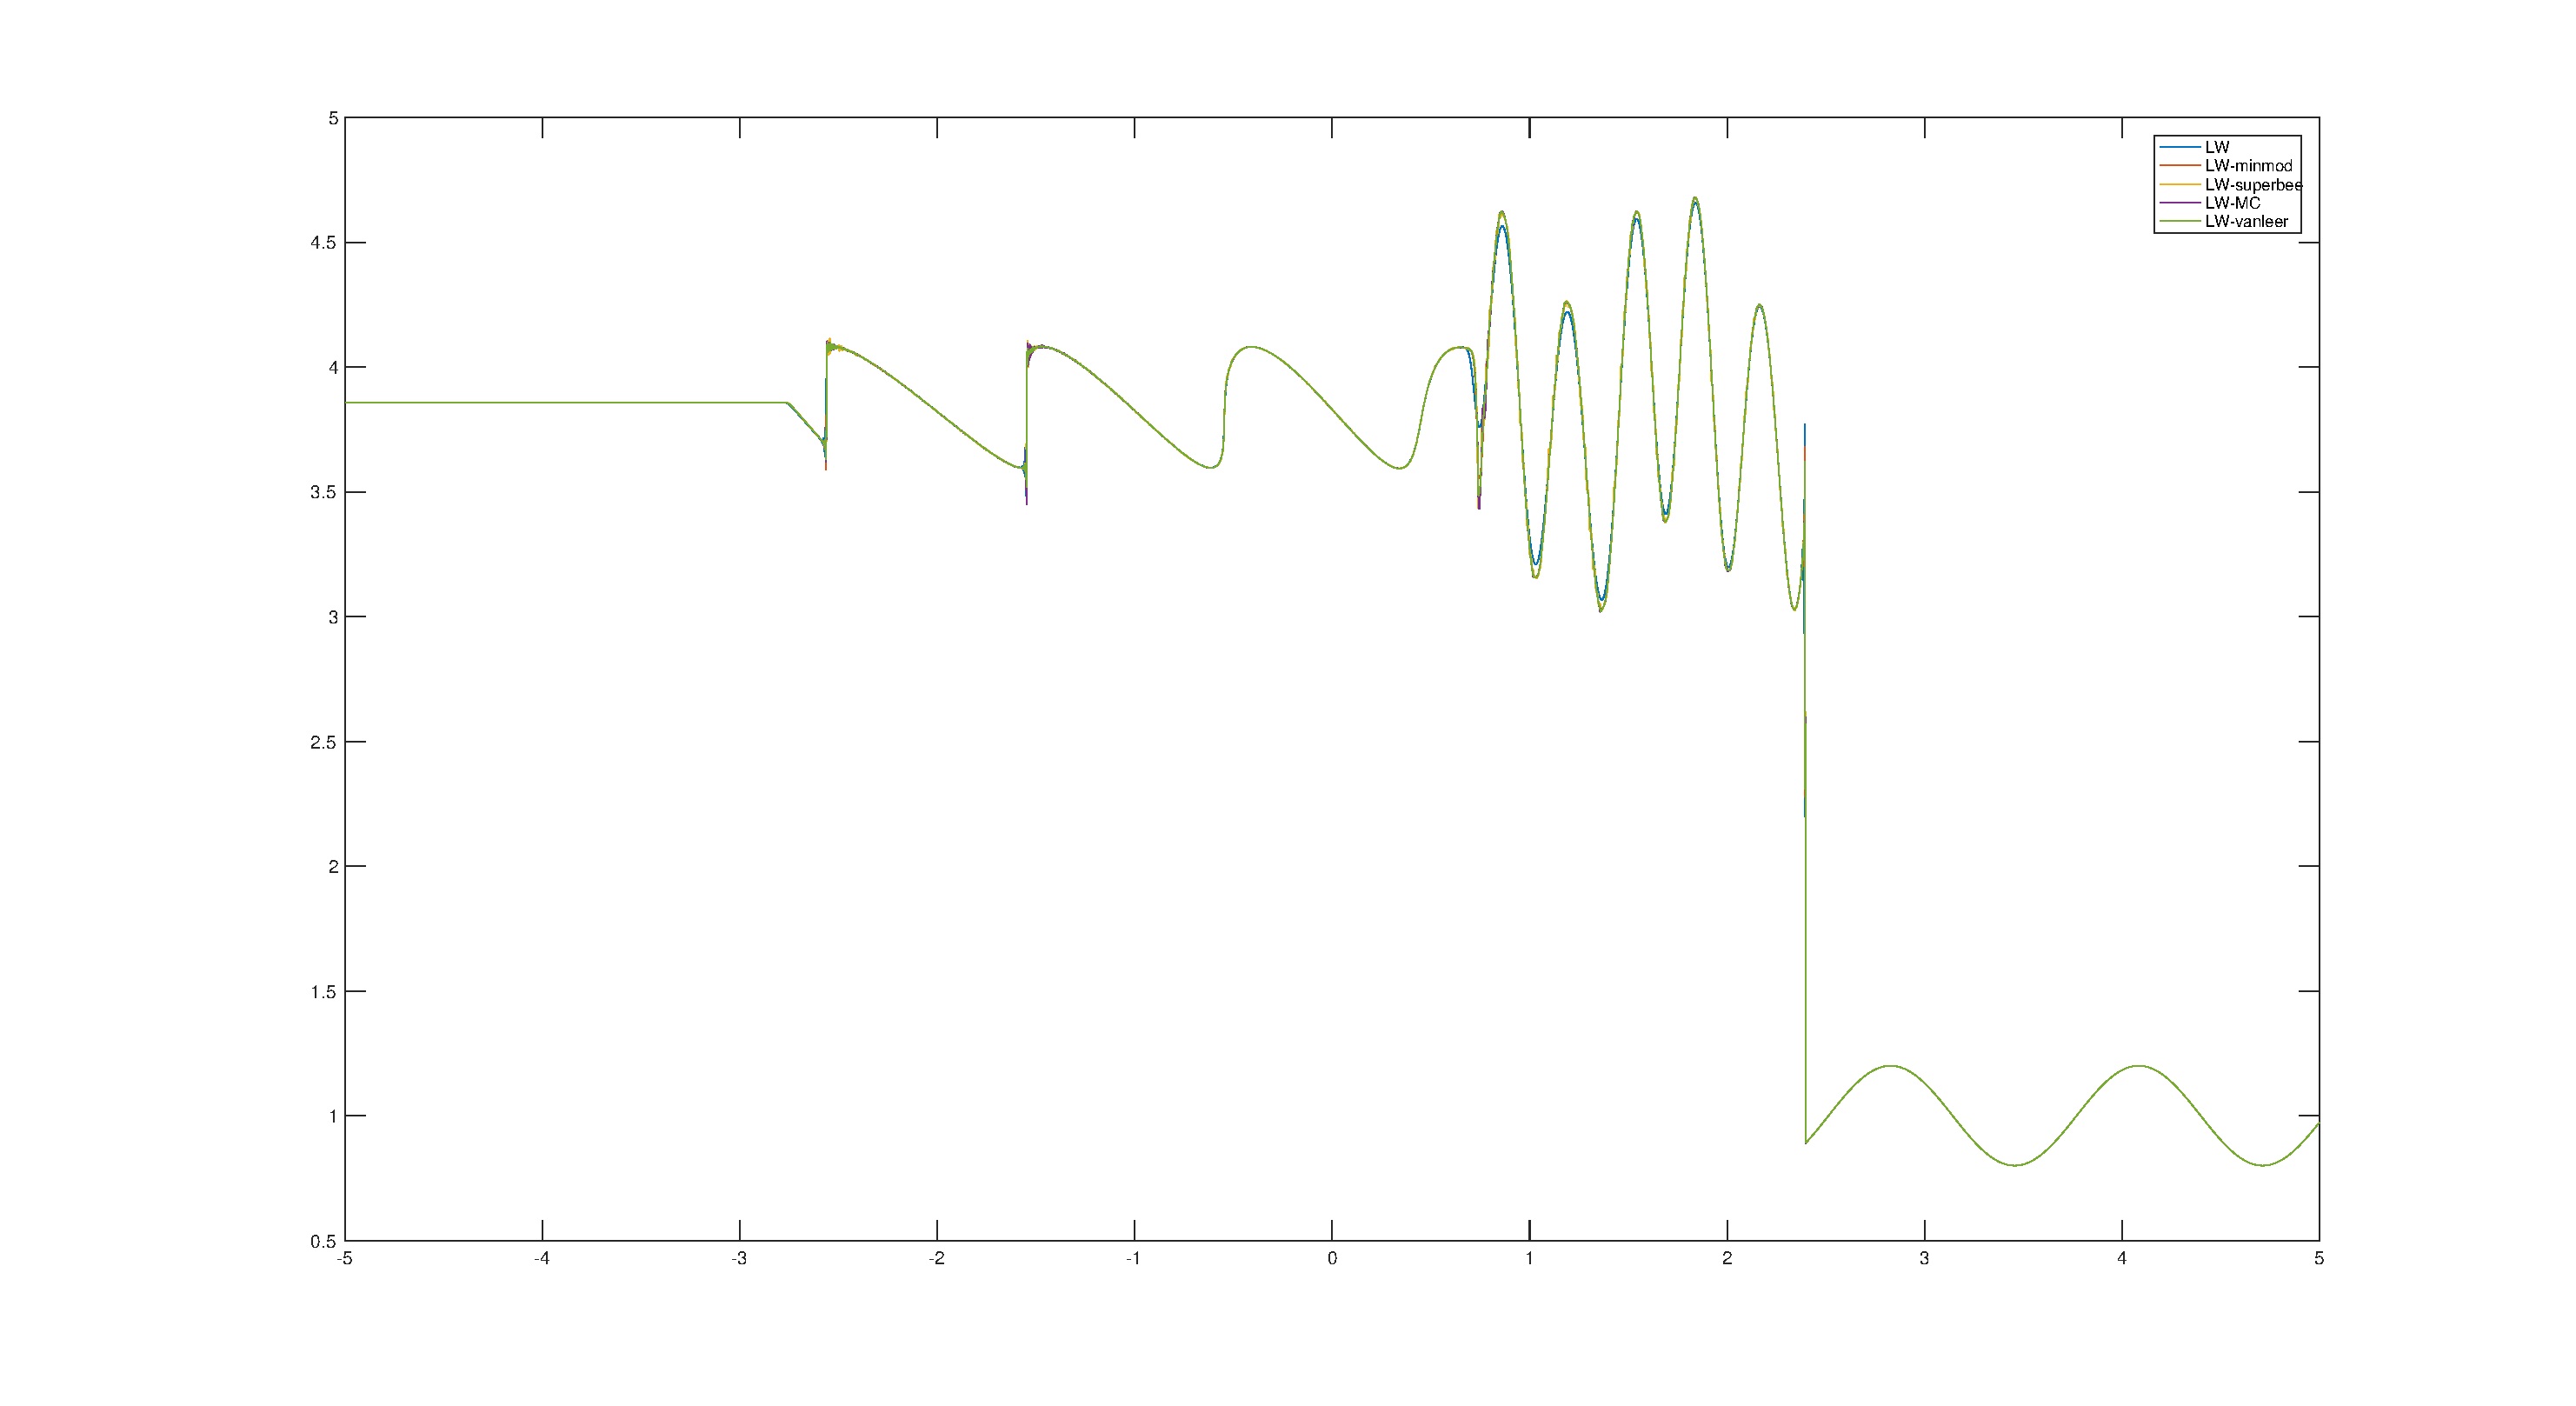
\includegraphics[width=\textwidth]{./images/EulerShu-LW.eps}
    \caption{Osher-Shu问题,LW数值通量}
  \end{center}
\end{figure}

\begin{figure}[H]
  \begin{center}
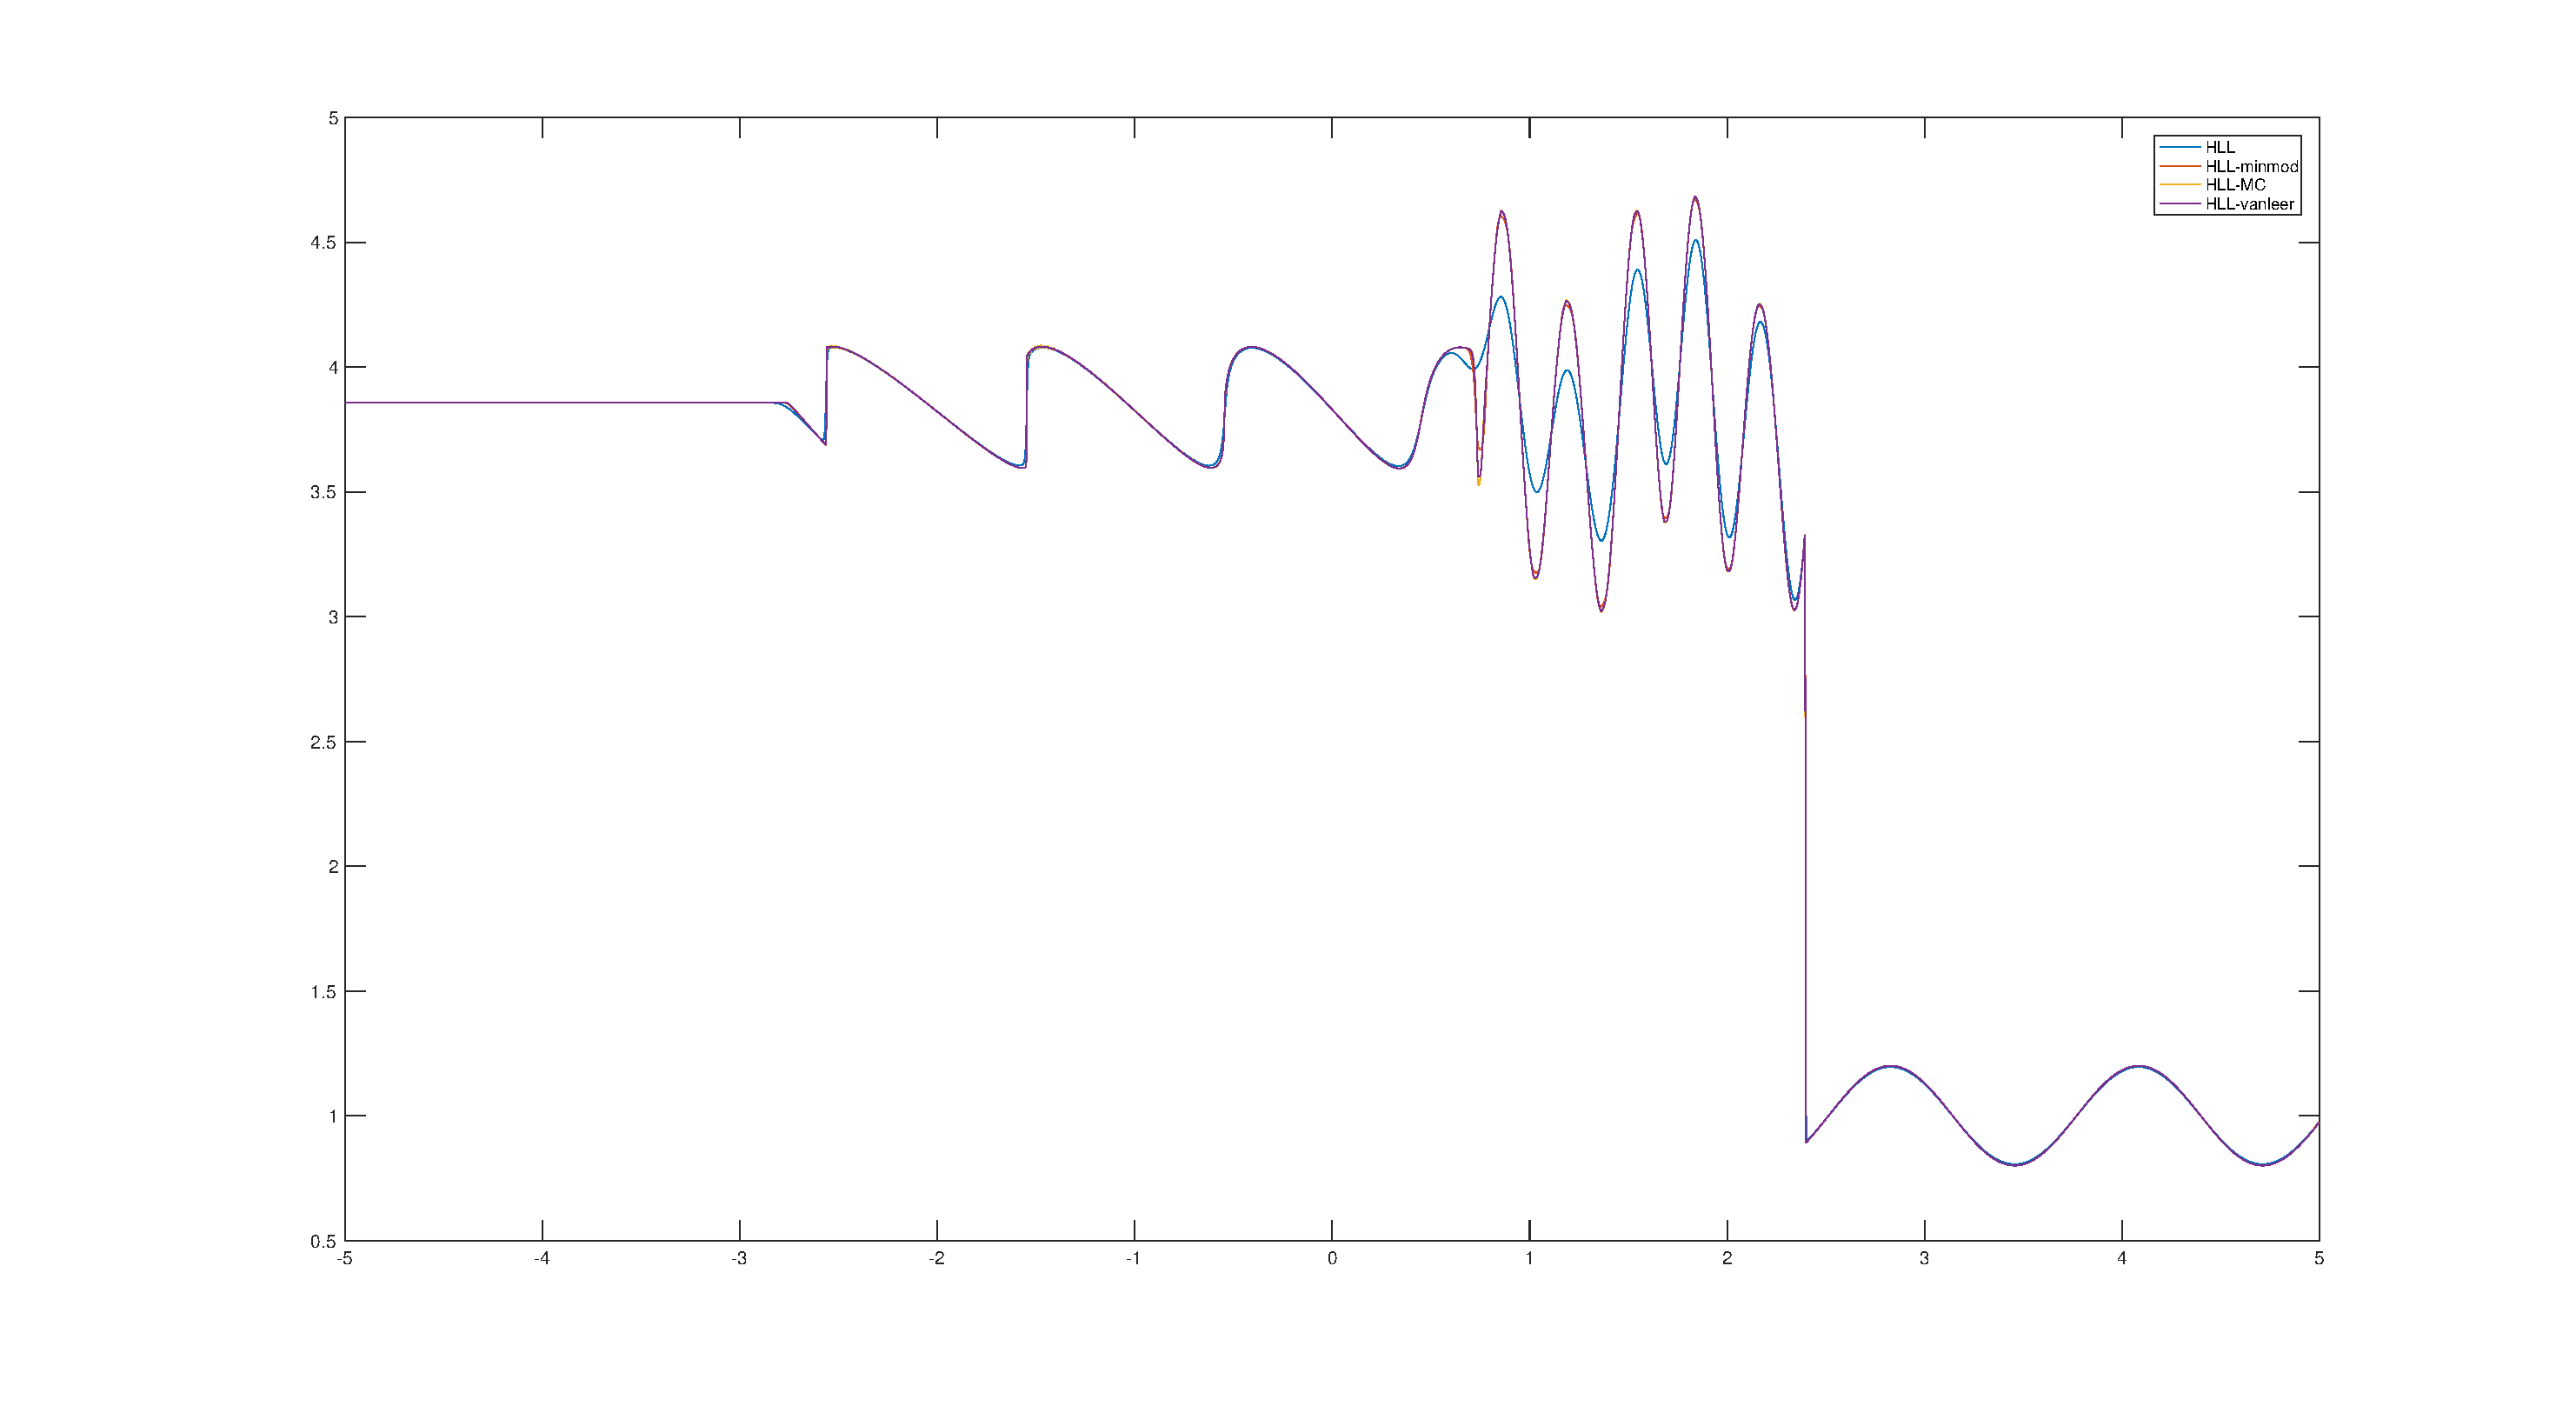
\includegraphics[width=\textwidth]{./images/EulerShu-HLL.eps}
    \caption{Osher-Shu问题,HLL数值通量}
  \end{center}
\end{figure}
\begin{figure}[H]
  \begin{center}
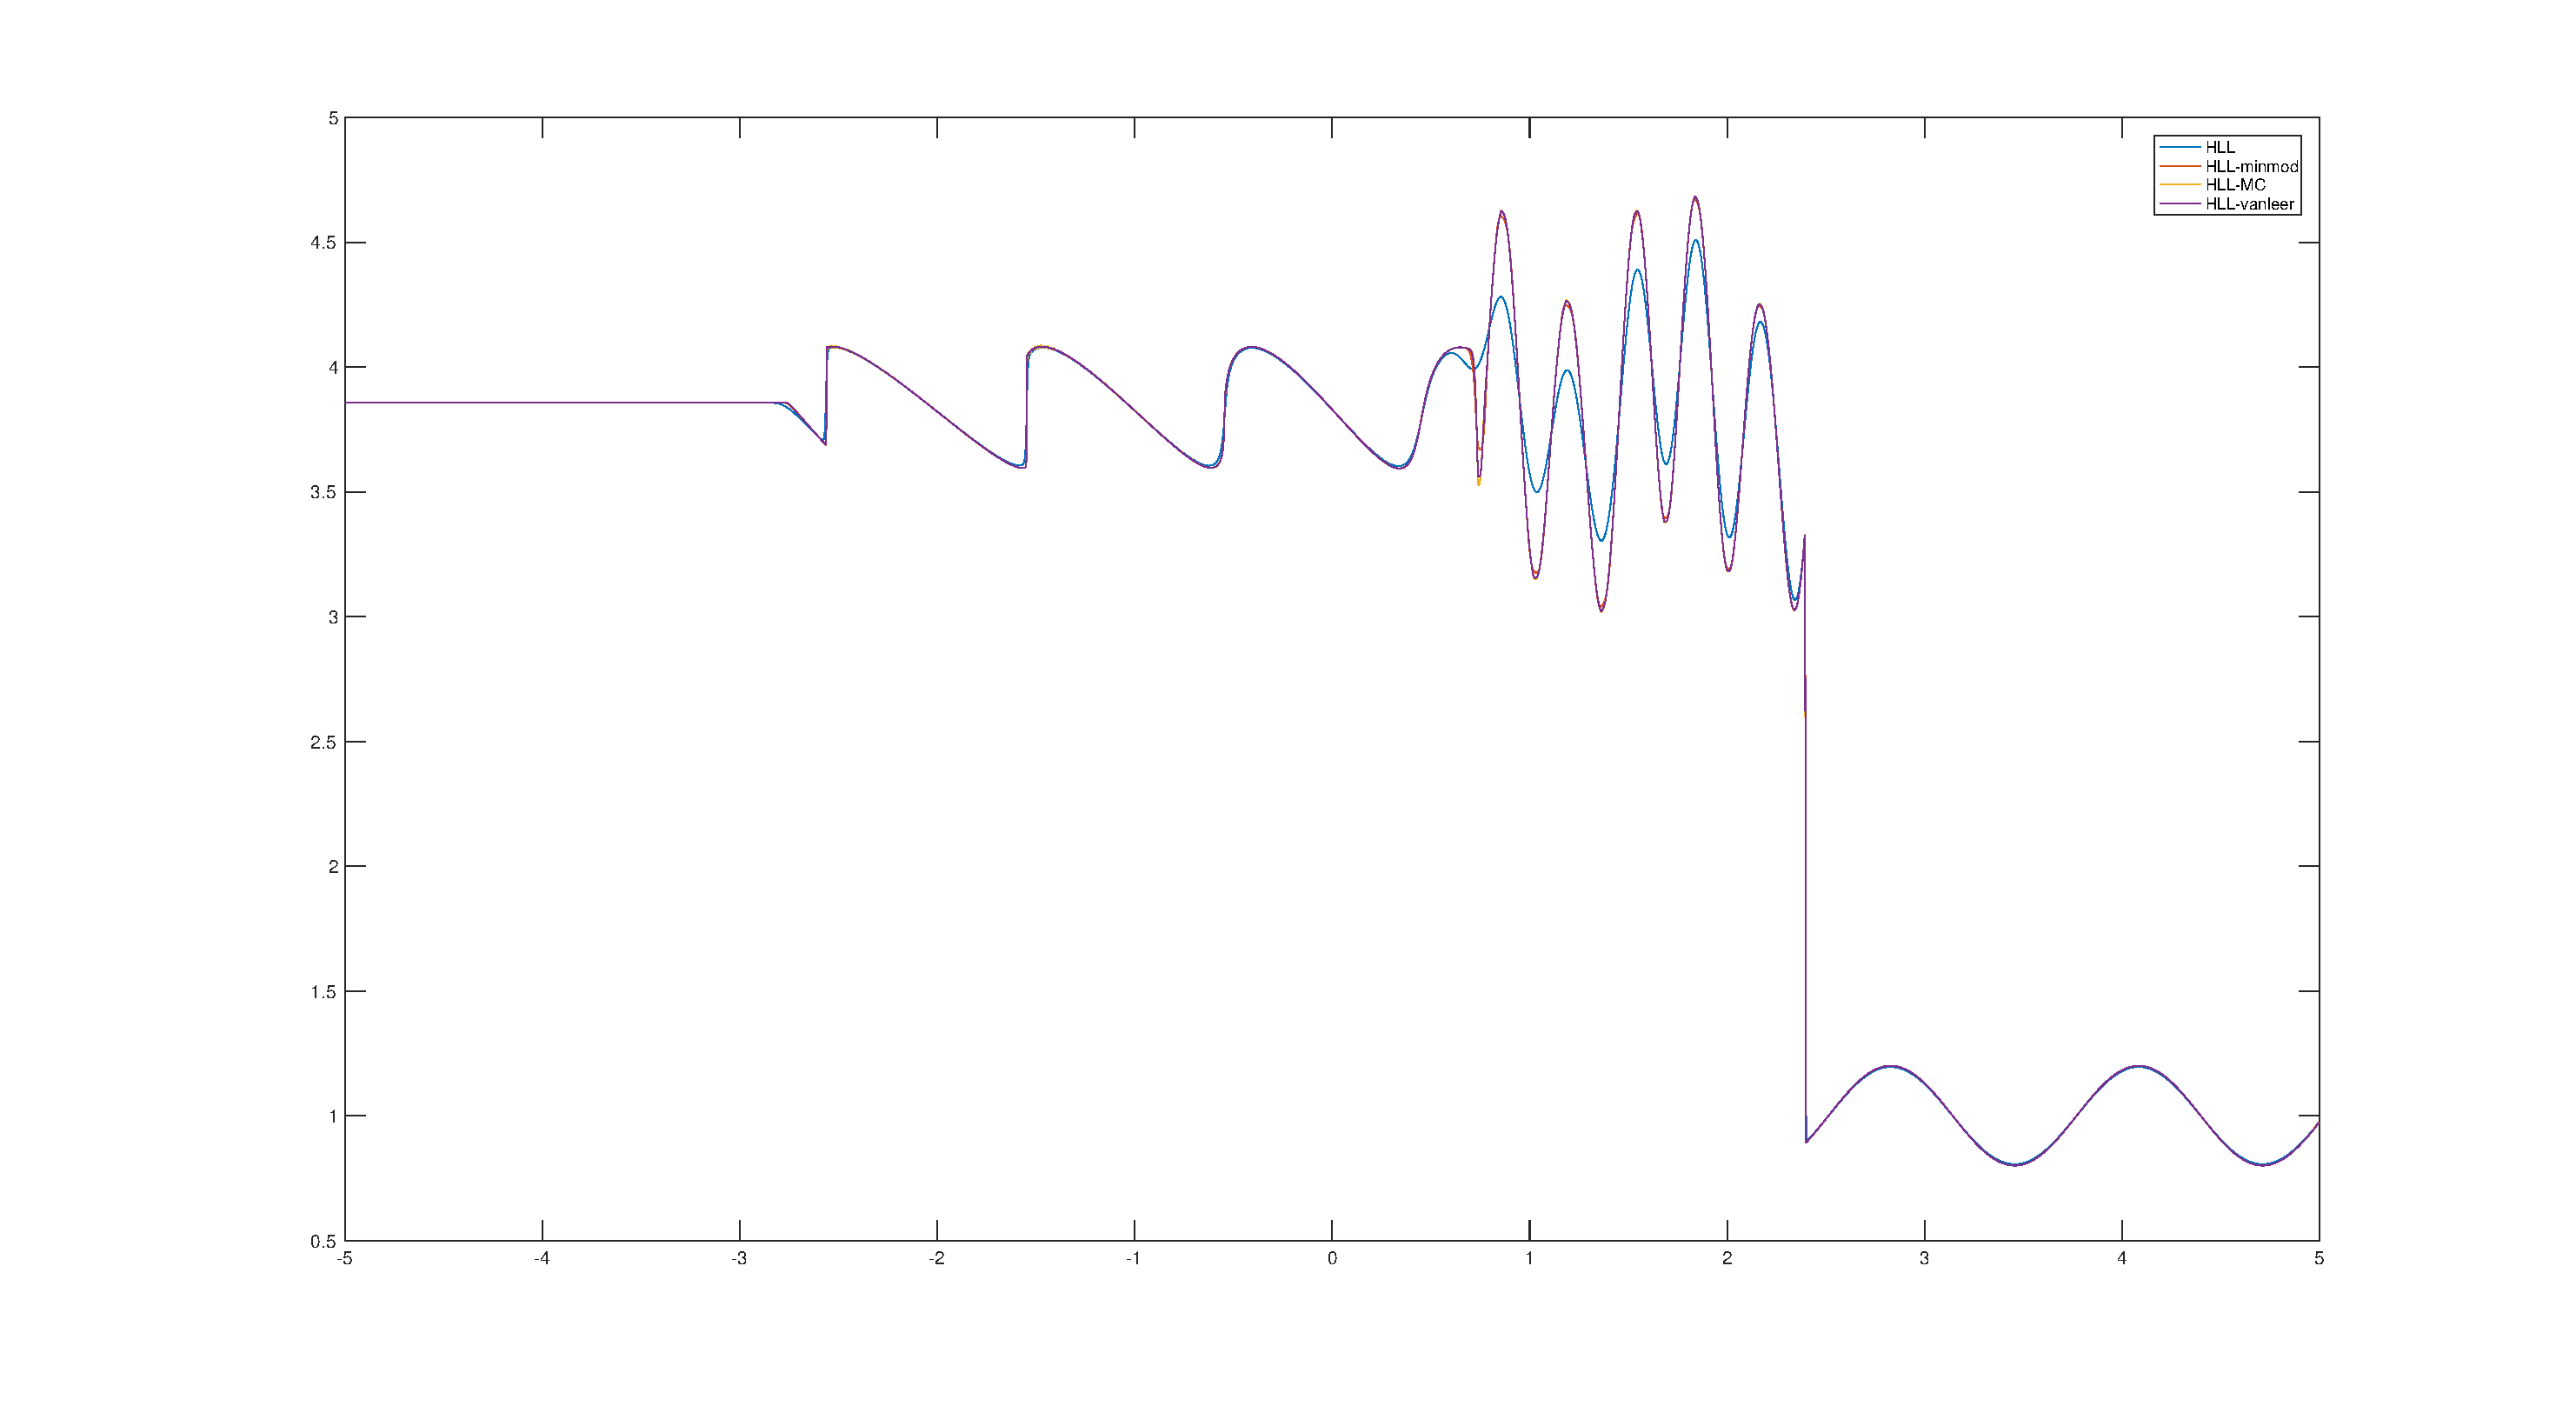
\includegraphics[width=\textwidth]{./images/EulerShu-HLL.eps}
    \caption{Osher-Shu问题,HLLC数值通量}
  \end{center}
\end{figure}
注意到这里的HLL和HLLC数值通量在superbee斜率限制器下会出现解不收敛的情
形,故而无法画出图像。
\subsubsection{小结}
通过上述实验,我们可以总结得到minmod通量较为保守,是TVD的但同时也有较
大的耗散;superbee通量较为激进,不是TVD的,而且容易将波形算为方波;MC和
vanleer在试验中显得较为出色,相比minmod具有更好的去耗散性质,但有时也
将出现数值解不收敛的情况,在下文的2维算例中,采用MC格式与HLL通量,无法
得到收敛的解。

综上所述,保守的通量和限制器能够得到收敛的解,但同时也带来耗散。
\subsection{二维问题}
接下来我们利用有限体积格式计算一些经典的二维算例。
\subsubsection{双马赫反射问题}
\begin{itemize}
  \item 计算区域$[0,4]\times[0,1]$
  \item 初值:$U_L=(8,57.1597,-33.0012,563.544)^T,U_R=
    (1.4,0,0,2.5)^T$。在$y=\sqrt{3}(x-\frac 16)$左侧为$U_L$,右侧为
    $U_R$。
  \item 边界条件:\\
    左边界:$U_L$的入流边界条件。 \\
    右边界:出流边界条件。 \\
    下边界:在$(0,\frac 16)$左侧为$U_L$入流边界条件,右侧为反射边界条件。\\
    上边界:入流边界条件,在$x=\frac 16+\frac{20t}{\sqrt{3}}$左侧为
    $U_L$,右侧为$U_R$。
\end{itemize}
下图为$t=0.2$时刻的密度等值线图。
\begin{figure}[H]
  \begin{center}
    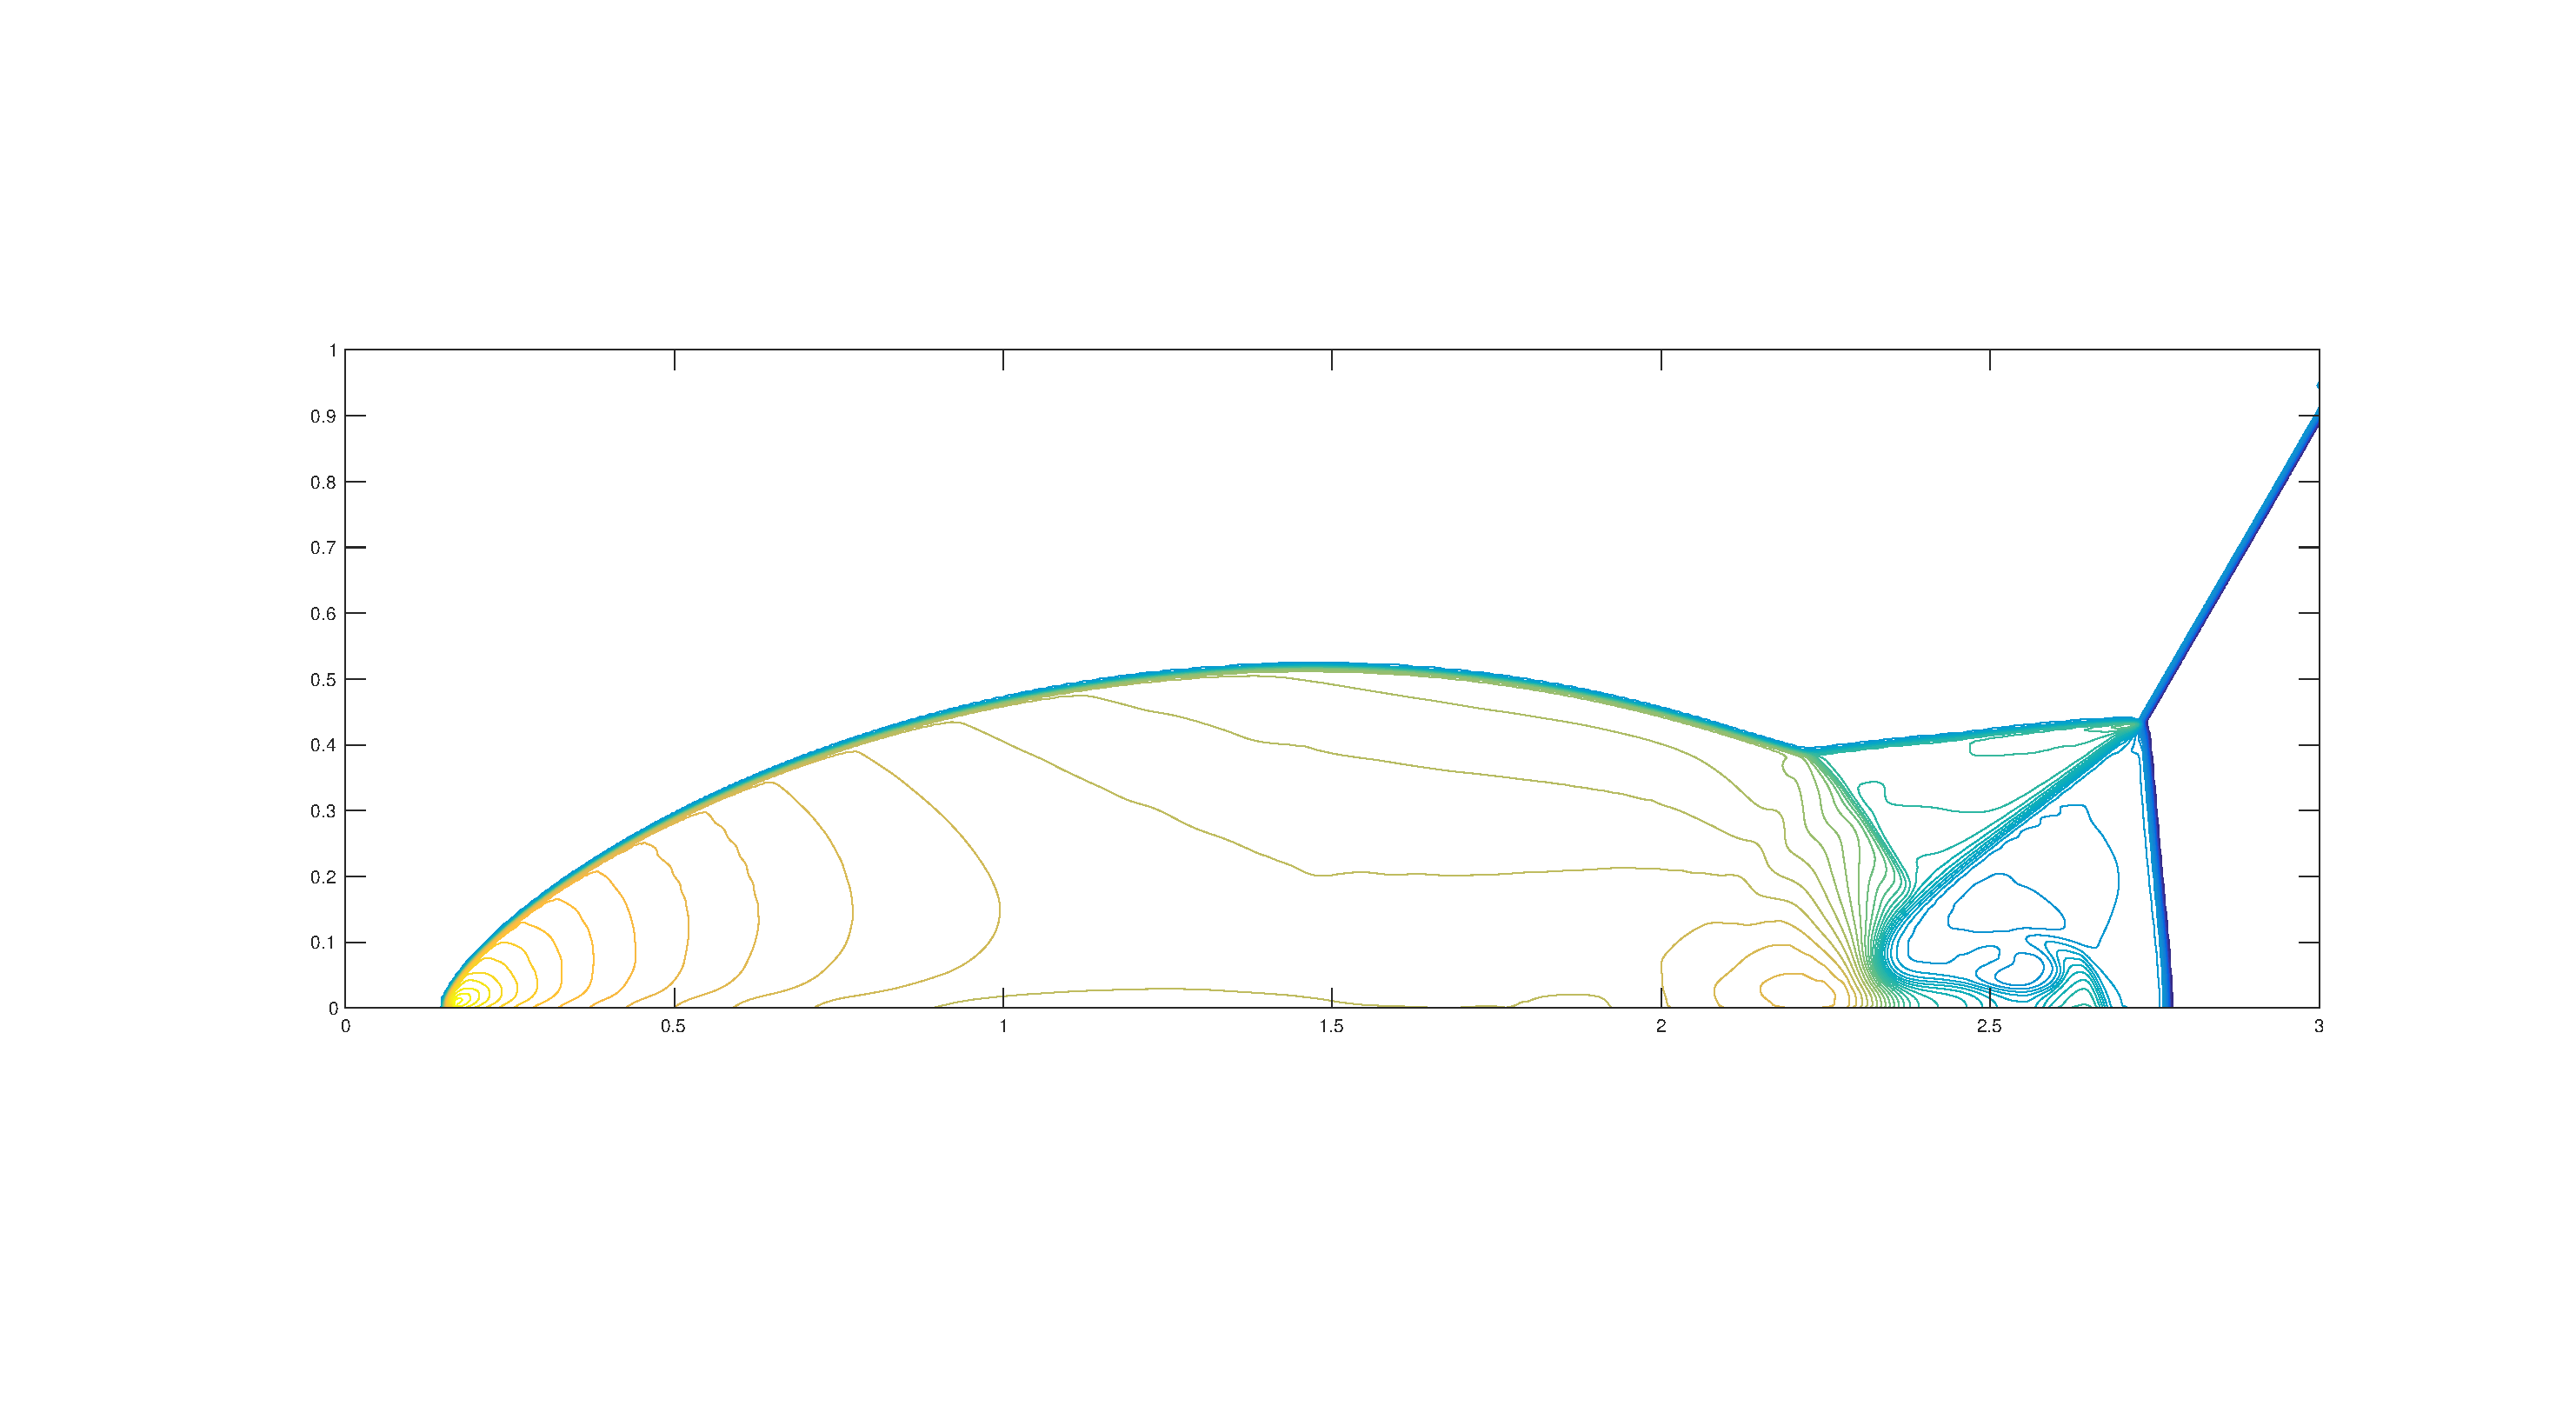
\includegraphics[width=\textwidth]{./images/MachReflection-960-240-HLL-minmod.eps}
  \end{center}
\end{figure}
\vspace{-3cm}
\begin{figure}[H]
  \begin{center}
    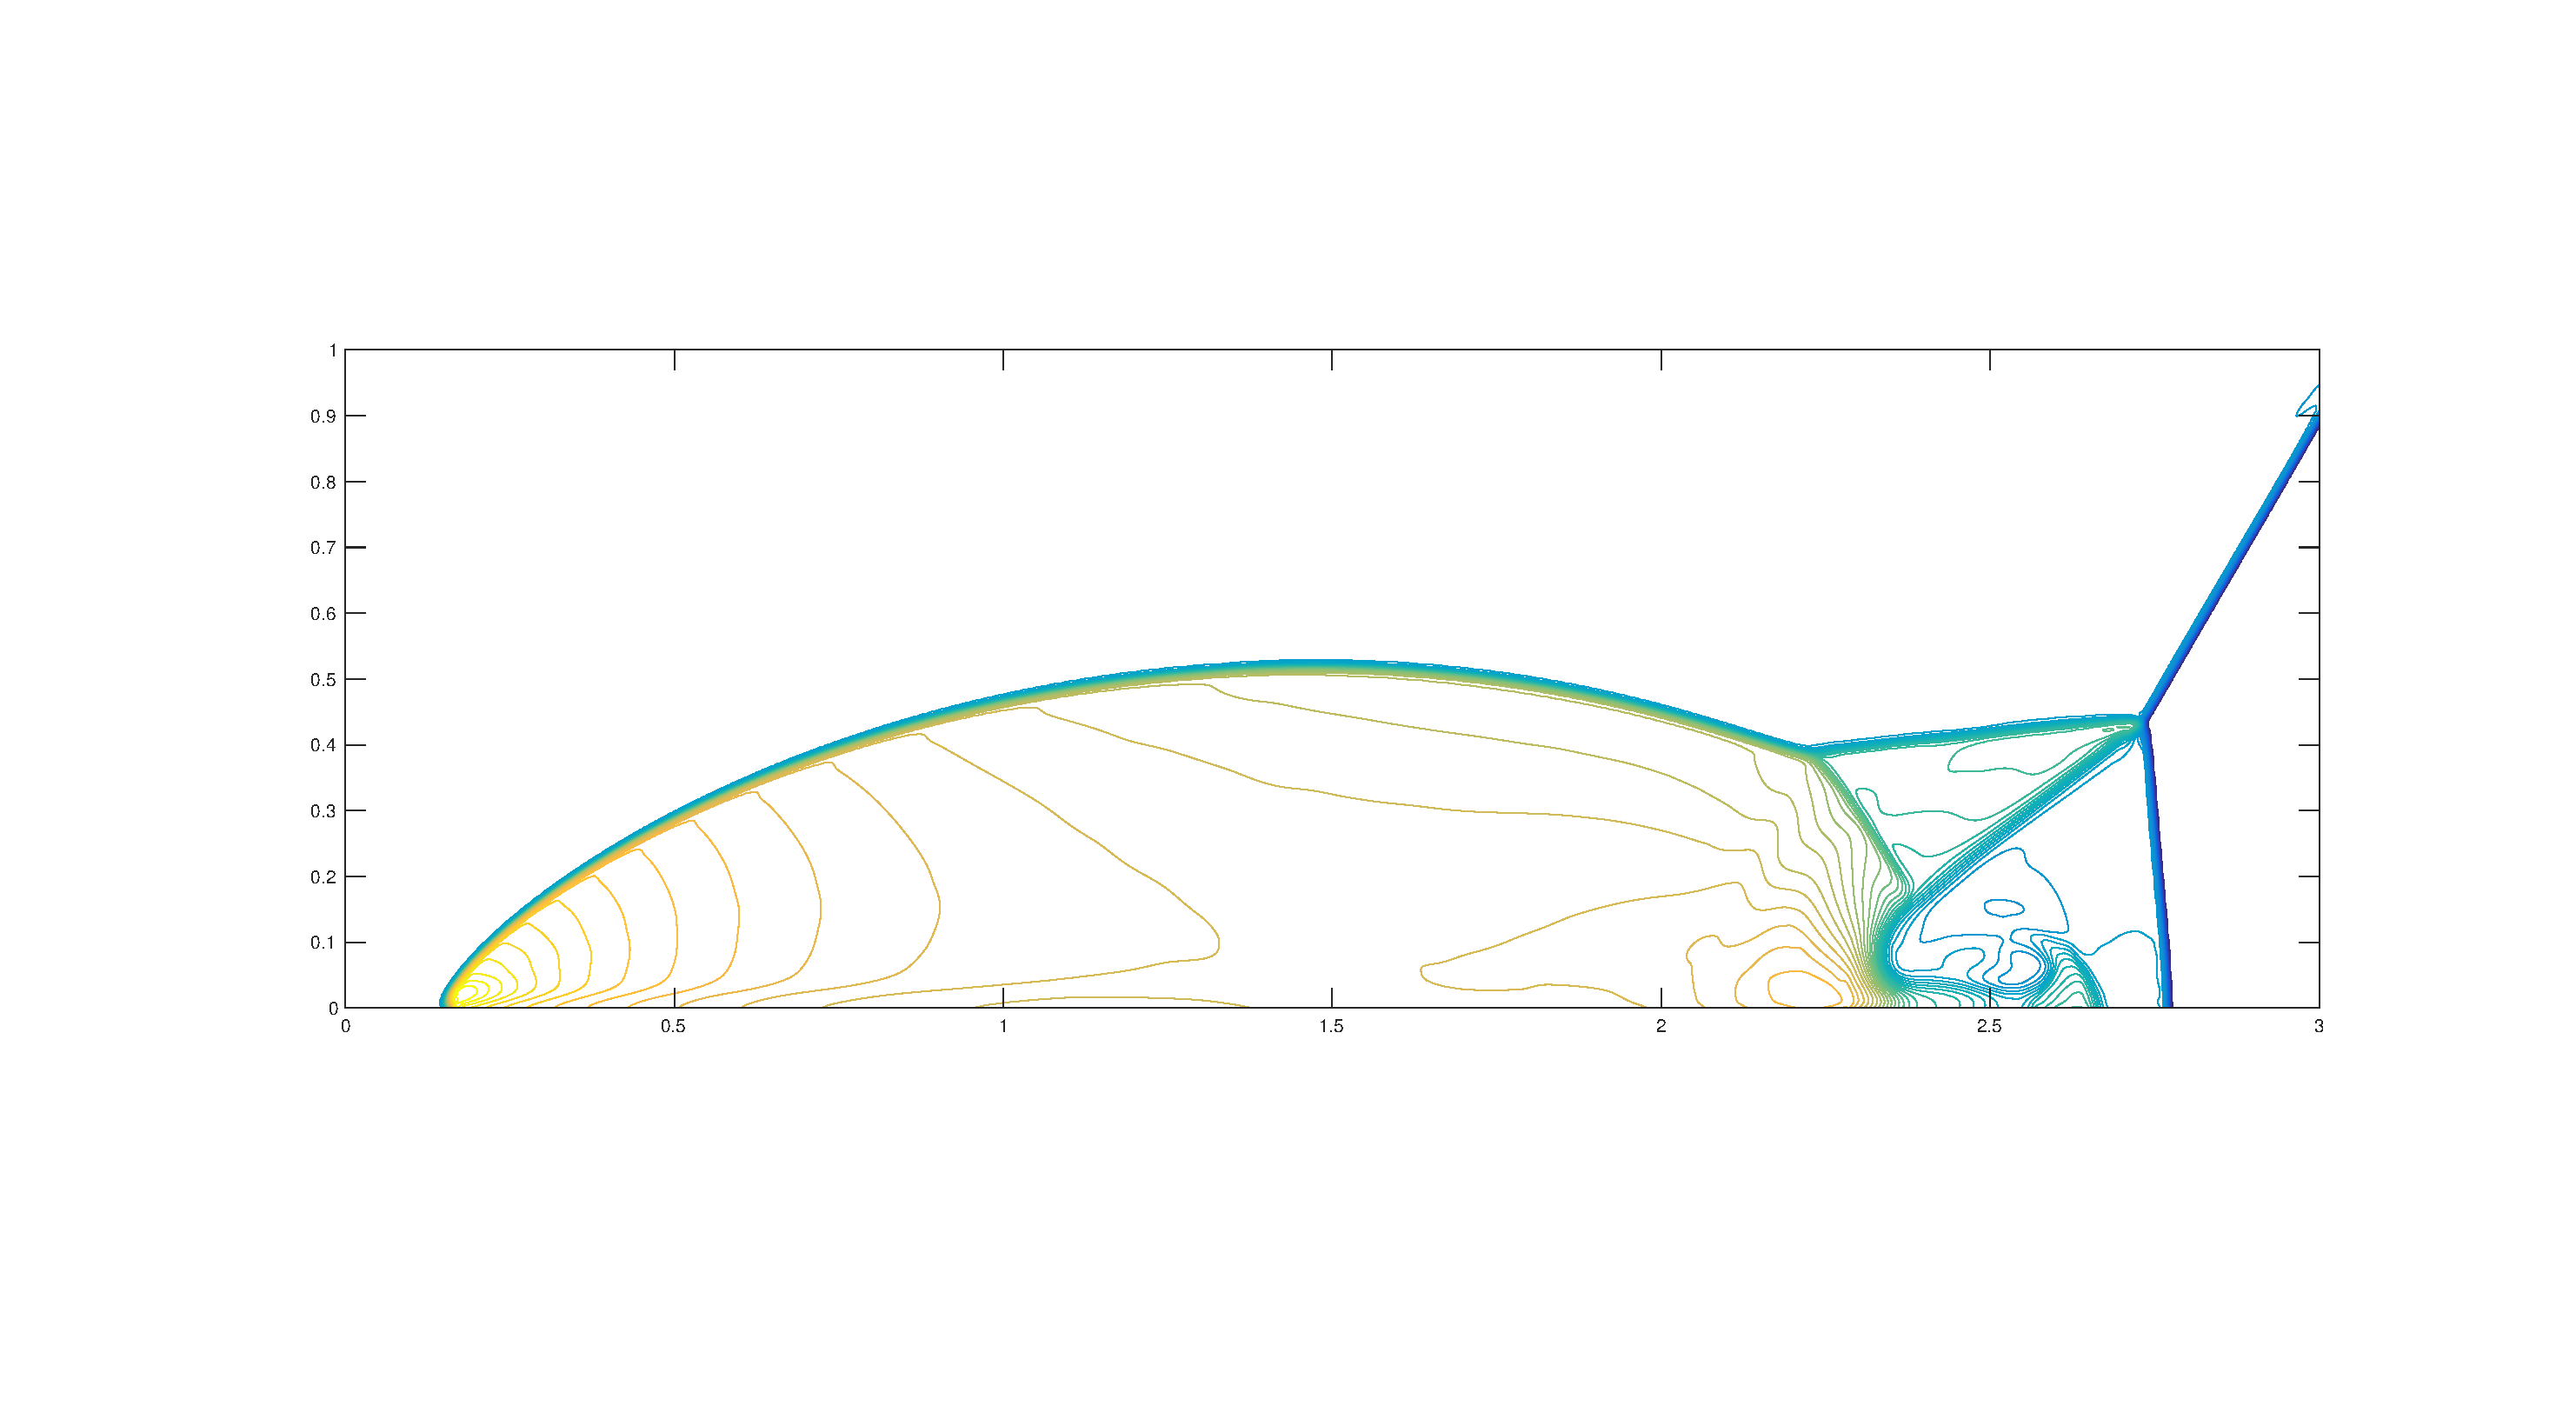
\includegraphics[width=\textwidth]{./images/MachReflection-960-240-LF-vanLeer.eps}
  \end{center}
\end{figure}
这里采用的数值通量和斜率限制器分别为HLL-minmod和
LF-vanleer.计算的$h=\frac{1}{240}$.

可见这儿的广义MUSCL格式能够大致给出问题的数值解,但对于右下角的精细结
构尚不能给出。右下角精细的波结构需要更高阶的重构方式来计算
(ENO和WENO重构方法)。 
\subsubsection{前台阶问题}
\begin{itemize}
  \item 计算区域$[0,3]\times[0,1]$。
  \item 初值条件$(\rho,u,v,p)=(1.4,3,0,1)$
  \item 边界条件:上下和台阶处为反射边界条件,
    左侧为入流边界条件,右侧为出流边界条件。
\end{itemize}
下图为$t=4$时的密度等值线图。
\begin{figure}[H]
  \begin{center}
    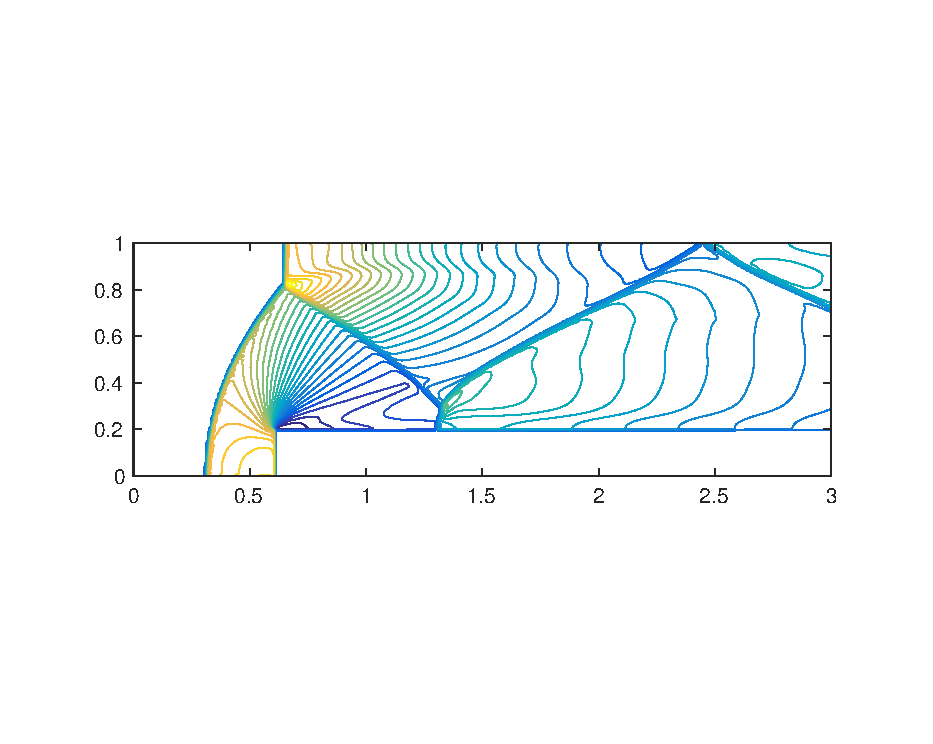
\includegraphics[width=\textwidth]{./images/ForwardStep-300-100-HLL-minmod.eps}
  \end{center}
\end{figure}
\vspace{-4cm}
\begin{figure}[H]
  \begin{center}
    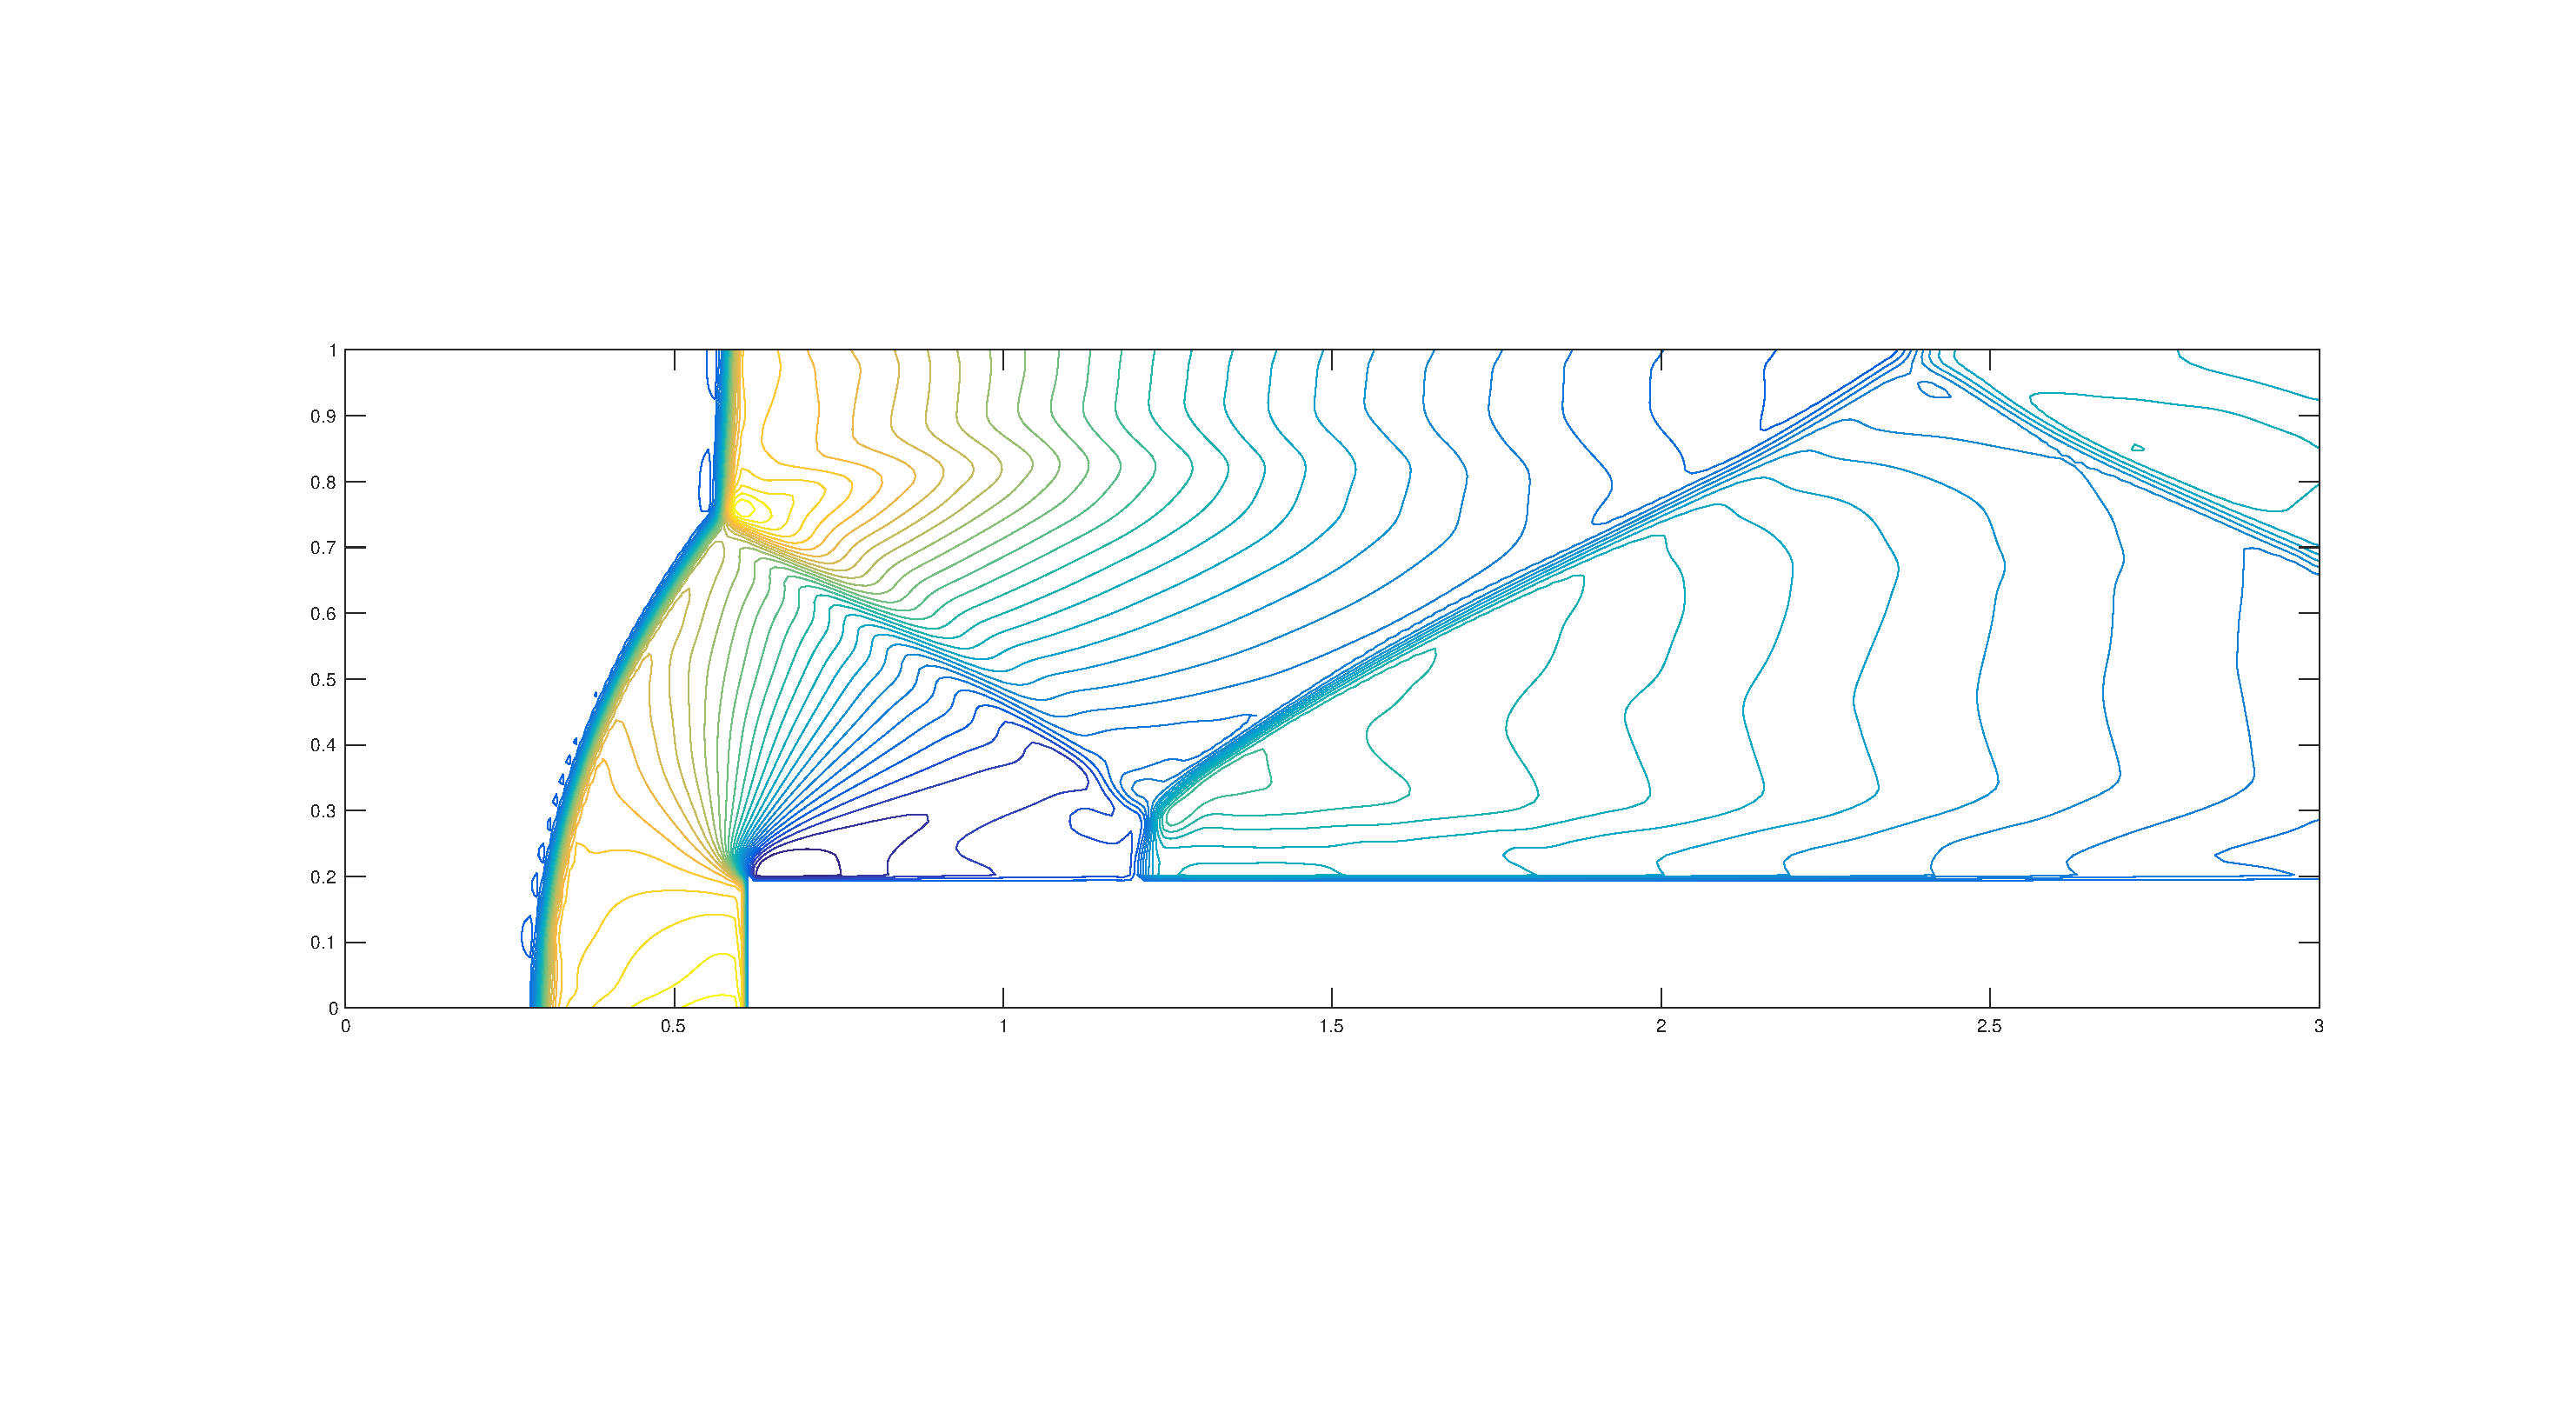
\includegraphics[width=\textwidth]{./images/ForwardStep-300-100-LF-MC.eps}
  \end{center}
\end{figure}
这里采用的数值通量和斜率限制器分别为HLL-minmod和LF-MC,计算采用的
$h=\frac{1}{100}$。
和双马赫问题一样,该问题的解也有一定的波结构,但不够精细。

\section{代码说明}
fvm1d与fvm2d分别为一维和二维的有限体积格式代码,config.h中可以修改
CFL条件数和设置(包括针对的问题,是否重构与对应的斜率限制器,以及是否采用3阶
Runge-Kutta方法),修改所采用数值通量需要进入fvm1d.cpp和fvm2d.cpp修改。
网格参数和终止时间由命令行参数传入。
\section{总结}
我们采用了广义MUSCL格式,对常见的数值通量格式和斜率限制器进行实验,比
较了他们的异同。可见斜率限制器和数值通量的保守和耗散是同时存在的。对于
不同的具体问题,我们需要采用不同的数值通量方法和斜率限制器,以保证在解
收敛的条件下尽量减少解的耗散。


\end{document}
